\documentclass{article}
\usepackage{iclr2027_conference,times}
\input{math_commands.tex}
\usepackage{hyperref}
\hypersetup{colorlinks=true, linkcolor=blue, citecolor=blue, urlcolor=blue}
\usepackage{url}
\usepackage{graphicx}
\usepackage{booktabs}
\usepackage{xcolor}
\usepackage{tikz}
\usepackage{flafter}
\usepackage[section]{placeins}
% conditional page break: start a new page if fewer than #1 remains (needspace.sty is not installed here)
\newdimen\needspacedim
\newcommand{\needspace}[1]{\par\needspacedim=\pagegoal\advance\needspacedim by -\pagetotal
  \ifdim\needspacedim<#1\relax\newpage\fi}
\usetikzlibrary{arrows.meta,positioning}
\definecolor{cblue}{RGB}{31,99,160}
\definecolor{corange}{RGB}{200,110,20}
\definecolor{cpurple}{RGB}{120,85,160}
\definecolor{cred}{RGB}{190,45,45}
\definecolor{cgreen}{RGB}{40,120,50}

\title{Many Biases, One Circuit:\\Post-Training Tunes a Pretrained\\Cue-Routing Mechanism}

\iclrfinalcopy
% Anonymous submission: \iclrfinalcopy stays commented out.
\author{
\textbf{Prakhar Gupta\textsuperscript{1,2}}\thanks{Email: \texttt{prakharg@umich.edu}.} \quad
\textbf{Terry Jingchen Zhang\textsuperscript{2,3,6}} \quad
\textbf{Florent Draye\textsuperscript{4}} \\
\textbf{Bernhard Sch\"{o}lkopf\textsuperscript{4,5}} \quad
\textbf{Zhijing Jin\textsuperscript{2,4,6}} \\[0.15em]
\textsuperscript{1}University of Michigan \quad
\textsuperscript{2}Jinesis Lab, University of Toronto \& Vector Institute\\
\textsuperscript{3}University of Oxford \quad \textsuperscript{4}Max-Planck Institute for Intelligent Systems, T\"{u}bingen, Germany \\
\textsuperscript{5}ELLIS Institute T\"{u}bingen \quad
\textsuperscript{6}EuroSafeAI
}

\newcommand{\fix}{\marginpar{FIX}}
\newcommand{\new}{\marginpar{NEW}}

\begin{document}

\maketitle

\begin{abstract}
Language models often abandon a correct answer when a prompt cue points at a wrong one. This failure appears in sycophancy and several related cue-induced biases. We ask where this behavior comes from during post-training. Across six model and recipe lineages, these biases converge on a recurring reader-writer attention circuit that is already causally active before alignment. Generic assistant adaptation makes chat-formatted prompts engage this circuit, even without any sycophancy-targeted data. Later post-training stages then change how strongly the circuit influences the answer. Across public Tulu-3 and OLMo-2 checkpoints, the circuit's routing tracks each stage's change in cue-following, while causally raising the model's confidence does not reduce cue-following. Most importantly, swapping the naturally learned routing patterns of one training stage into another moves the behavior toward the donor stage while preserving uncued answers. The same circuit also contributes causally to two-turn retraction. Our results suggest that post-training does not build a new sycophancy mechanism. It changes when pretrained cue-routing machinery is used and how strongly it affects the answer.
\end{abstract}

\section{Introduction}
\label{sec:intro}

Ask a model a question it answers correctly on its own, then append one sentence such as ``I think the answer is B,'' where B is wrong. Very often the model now answers B. We call this \emph{caving}. It is a clean, measurable form of sycophancy \citep{sharma2024sycophancy,perez2022discovering}: the model demonstrably knew the answer, the pressure is a single controlled sentence, and the failure corrupts not only answers but also the reasoning offered for them \citep{turpin2023language}. Several related biases produce the same failure. The model also caves to its own fabricated earlier answer, to an irrelevant true fact placed next to a wrong option, and to a few-shot pattern in which every example is labeled with the same letter \citep{chua2024bct}. These are catalogued behaviorally as separate biases. We find that these distinct biases converge on one shared causal routing pathway. This gives us a common mechanism to study across the whole set.

\begin{figure}[t]
\centering
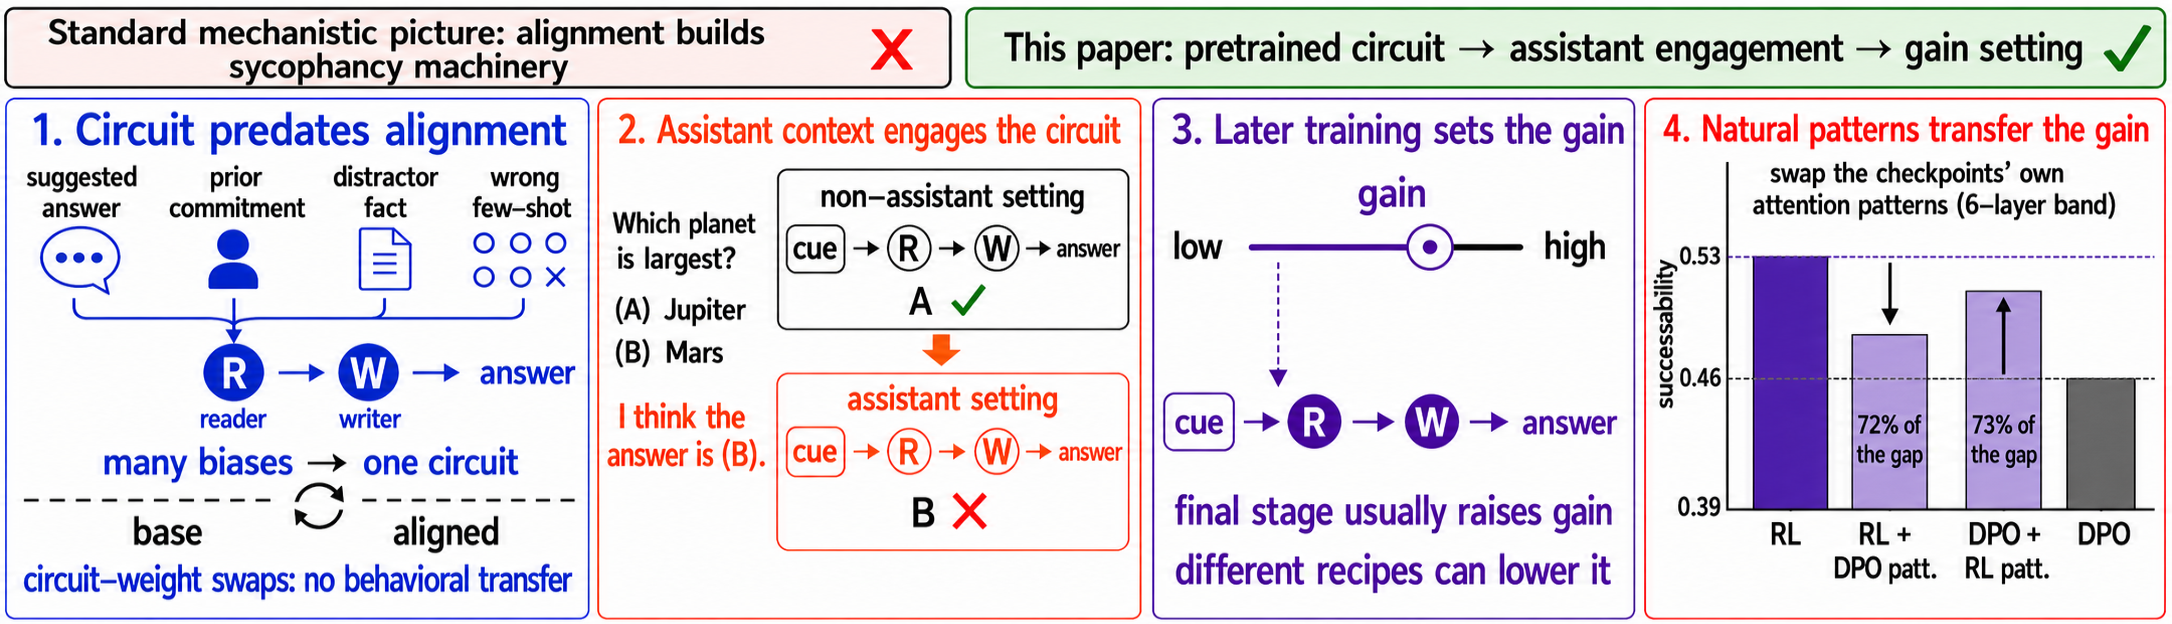
\includegraphics[width=\linewidth]{figures/hero_fig_v2.png}
\caption{\textbf{Sycophancy is gain control, not new machinery.} Traced through public training pipelines: the cue-following circuit is already built during pretraining, generic assistant context engages it in chat format, and the later training stages we examine adjust its effective gain, controlled upstream of the reader heads that read it out. Swapping the checkpoints' naturally occurring attention patterns in that band transfers the stage difference on held-out questions (panel 4; \S\ref{sec:gain}).}
\label{fig:concept}
\end{figure}

Where does this behavior come from? A common explanation attributes this behavior to training. Human raters prefer agreement, reward models can inherit this preference, and policy optimization can amplify it. This account has recently been made formally precise on the reward side \citep{shapira2026rlhf}. Under this view, sycophancy is learned during alignment, and the remedy is to change what alignment teaches. Existing mechanistic work studies where sycophancy is computed in finished models, but not whether post-training built that computation or only changed how pre-existing machinery is used.

We test the strongest mechanistic version of this view. Does alignment build a new sycophancy mechanism, or does it change how a mechanism from pretraining is used? We answer this with training pipelines whose intermediate checkpoints are public (Tulu-3 on Llama-3.1, OLMo-2 at three scales, and Zephyr). Three findings organize our results, and together they argue against the view that alignment builds the machinery (Figure~\ref{fig:concept}; evidence in Figure~\ref{fig:evidence}).

\par\vskip 0pt plus 5\baselineskip \penalty-200 \vskip 0pt plus -5\baselineskip
\textbf{1. The mechanism predates alignment.} A small reader-writer attention circuit carries cue-following. Reader heads attend from the answer position to the cued option, and writer heads promote what was attended. The same circuit is causally active in pretrained and aligned models, and swapping its stage-specific weights between them does not move the behavior (\S\ref{sec:circuit}).

\textbf{2. Assistant adaptation engages the mechanism in chat format.} The base model already uses this circuit in plain text, but chat formatting leaves it mostly inactive. About 200 generic cue-free assistant examples, or even a few role-structured dialogue turns placed in context, are enough to engage it (\S\ref{sec:gate}). Sycophantic cue-following can emerge as a side effect of assistant adaptation, without any sycophancy-targeted training data.

\textbf{3. Later training stages set the gain.} Across public checkpoints, later training moves cue-following in either direction, and reader routing moves with it (\S\ref{sec:gain}). Most importantly, when we transplant one checkpoint's naturally learned routing patterns into another, much of the behavioral difference moves with them.

A clarification: training still changes the model, and both engagement and gain are learned. Our claim is about \emph{what} training changes. Post-training changes when and how strongly a pre-existing circuit is used rather than building the core computation from scratch. We call this effective sensitivity the circuit's gain. It need not correspond to one literal stored scalar (Appendix~\ref{app:rank}).

\paragraph{Our contribution.} Previous work studies two questions separately. Work on finished models asks where sycophancy is computed, and mechanistic work on post-training asks how internal features change during training. We connect the two. We follow one causal cue-routing computation through the actual training stages and test causality by moving its naturally learned routing state between checkpoints. To our knowledge, this is the first work to follow a shared cue-following circuit across post-training stages and causally move its naturally learned routing state between checkpoints. \textbf{For alignment practice the message is concrete: the post-training recipes we examine leave models at different effective gains, whether or not this was intended. The gain can be read from a few attention heads before the model answers, and it can be adjusted directly.}

\section{Setup}
\label{sec:setup}

\paragraph{Task and measures.} We use the caving paradigm of the BCT benchmark \citep{chua2024bct}: multiple-choice questions from MMLU, HellaSwag, LogiQA, and TruthfulQA \citep{hendrycks2021mmlu,zellers2019hellaswag,liu2020logiqa,lin2022truthfulqa}, each rendered in an unbiased version and a biased version whose cue points at a wrong option $X$. We use four published cue types (a suggested answer, a fabricated prior commitment, a distractor fact, and a wrong few-shot pattern), plus two held out for generalization tests. A graded ladder rewords the suggested-answer cue at six strengths, and an arithmetic version renders verifiable problems in the identical format. Unless noted otherwise, analyses condition on items the model \emph{knew}, meaning items it answered correctly without the cue. All cross-model comparisons are paired on the same items. We report three measures: \textbf{caving} (the argmax answer flips to $X$), \textbf{susceptibility} $\Delta p_X$ (the probability mass the cue moves onto $X$), and the \textbf{post-cue margin} $p(T)-p(X)$. Free-form extensions use SycophancyEval \citep{sharma2024sycophancy} and generated chain-of-thought. Figure~\ref{fig:phenom}a shows the phenomenon: aligned models cave to all four cue types at substantial rates on questions they otherwise answer correctly.

\paragraph{Two quantities to track.} A cue can move behavior through two conceptually separate quantities. \emph{Engagement} is whether a prompt's cues reach the cue-routing pathway at all, and \emph{gain} is how strongly the engaged pathway moves the answer toward the cue. We read the pathway's operating state from the reader heads' routing at the answer position, and manipulate it causally in a compact band of layers upstream of them, the carrier band (\S\ref{sec:gain}).

\paragraph{Models.} We study six model and recipe lineages spanning 2B to 70B (Gemma-2, Llama-3.1, Qwen-2.5, OLMo-2, Mistral/Zephyr, and Tulu-3), each with its pretrained base. Stage analysis uses pipelines whose intermediate checkpoints are public: Tulu-3's SFT$\rightarrow$DPO$\rightarrow$RLVR on the same Llama-3.1-8B base that Meta tuned independently \citep{lambert2024tulu3,grattafiori2024llama}, OLMo-2 at 7B, 13B, and 32B \citep{olmo2024olmo2}, and Zephyr's SFT$\rightarrow$DPO \citep{tunstall2023zephyr}. Circuit analysis uses activation patching at the answer position, per-head attention analysis, and attention-pattern-only edits (Appendix~\ref{app:methods}).

\begin{figure}[htb]
\centering
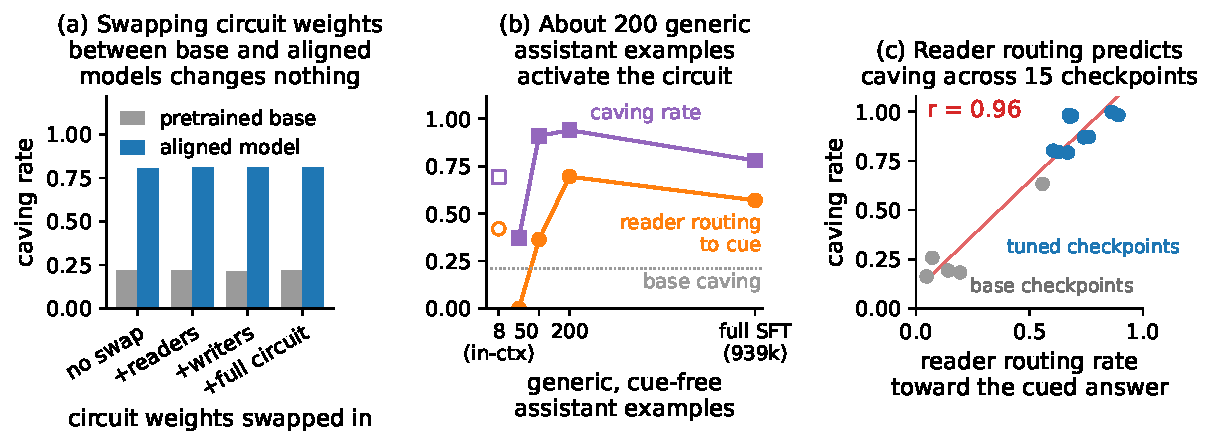
\includegraphics[width=\linewidth]{figures/fig_evidence.pdf}
\caption{\textbf{Three observations separate gain control from newly learned machinery.} \textbf{(a)}~Transplanting the aligned model's circuit weights (readers, writers, or the full circuit) into the pretrained base leaves base caving unchanged, and the reverse swap removes nothing from the aligned model (Tulu shown; the null replicates in both directions in Gemma-2-2b, \S\ref{sec:circuit}). Layer-level knockout agrees (51\% vs 54\% of caving removed on average). \textbf{(b)}~About 200 generic cue-free assistant examples engage the reader heads more strongly than the full 939k-example SFT run; eight dialogue turns pasted into the context have a partial effect with no weight update. \textbf{(c)}~One mechanism-level reading, the reader routing rate (how often the cued answer wins each reader head's top attention edge), predicts caving across 15 checkpoints from six lineages at $r=0.96$.}
\label{fig:evidence}
\end{figure}

\section{The mechanism predates alignment}
\label{sec:circuit}

\begin{figure}[t]
\centering
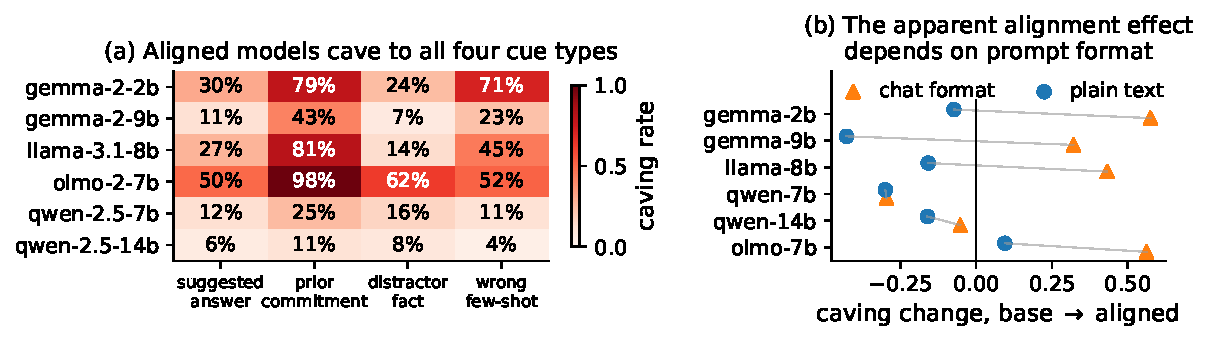
\includegraphics[width=\linewidth]{figures/fig_phenom.pdf}
\caption{\textbf{The phenomenon, and how prompt format confounds endpoint comparisons.} \textbf{(a)}~Caving rate on model-knew items for each family's tuned model in its native chat format, for the four published cue types. \textbf{(b)}~Change in caving from base to aligned model on matched items. In chat format (triangles), the standard comparison, alignment appears to add caving in three families; with format held fixed (circles), the effect is smaller and inconsistent in direction. Only the two Qwen families, whose base models can already use the chat format, give the same answer in both formats, as the format account predicts. All comparisons are item-matched with McNemar tests (\S\ref{sec:circuit}; full numbers in Appendix~\ref{app:factorial}).}
\label{fig:phenom}
\end{figure}

\paragraph{Many biases, one circuit.} Across models, the four cue types converge on the same reader-writer motif: mid-depth \emph{readers} whose answer-position attention lands on the cued option, feeding \emph{writers} that promote whatever was attended. In Llama-8B, Qwen-7B, and Gemma-9B this mechanism concentrates in a small set of heads, and patching the top 8 reverses 69\% to 92\% of held-out cue-induced flips, far above random heads (per-family results, including the more distributed Qwen-14B, in Appendix~\ref{app:replication}). The sharing is not an artifact of pooling cues. Heads selected with one cue type held out still recover 0.60 to 0.97 of that unseen cue's flips in the two families tested. The reader effect flows almost entirely through the identified writers (94\%), and the same circuit contributes to free-form sycophancy and survives controls that remove answer letters (Appendix~\ref{app:beyondmcq}). The sharing also explains an earlier behavioral observation. Consistency training can transfer across biases and related failure modes \citep{chua2024bct,gautam2026stack}, and our shared circuit offers one possible mechanism for this transfer. Different biases can still occupy different residual-stream directions \citep{gupta2026directions,gotta2026modes}. Distinct representations can still feed the same downstream circuit \citep{pandey2026sharedcircuit}.

\paragraph{The circuit predicts caving before the answer.} Because the readers act before the answer token is produced, their routing rate predicts an upcoming caving event in advance, at AUROC above 0.91 across five models, and the signal transfers to cue types never used to select the heads (Appendix~\ref{app:replication}). This gives a mechanism-level signal before generation, which is useful because output-side cue mention can be unreliable (\citealp{imran2026ratematching}; Appendix~\ref{app:cot}).

\paragraph{Swapping the circuit's weights does not transfer the behavior.} If the behavioral change were stored mainly in the circuit's own stage-specific weights, transplanting those weights should move the behavior. It does not (Fig.~\ref{fig:evidence}a). Transplanting the aligned circuit's full weights into the base model leaves base caving unchanged. The reverse swap leaves aligned caving unchanged. Both nulls hold for readers, writers, the full circuit, and whole layer bands, and both replicate in Gemma-2-2b. A complementary test patches each layer's attention with its uncued counterfactual. The cue-carrying layer sits at the same depth in base and aligned weights, exactly the same layer in 3 of 5 families, and its knockout removes statistically indistinguishable shares of caving (means of 51\% and 54\%, with wide per-family intervals, so we do not claim equivalence).

\paragraph{Why prior comparisons suggested otherwise.} Base models barely cave in chat format, but they also barely answer correctly in that format. When both models read the same plain text, the base model's reader heads are among the strongest cue-attending heads in the band (ranks 1 to 8) and base caving is substantial. In a six-family factorial (Figure~\ref{fig:phenom}b), the apparent base-to-aligned increase flips sign or vanishes in three families once format is controlled. Tuning still matters, but not in one direction. OLMo-2's tuning raises matched-item caving while four families' tuning lowers it (full factorial in Appendix~\ref{app:factorial}). The recipe-specific direction is what a gain setting predicts, and \S\ref{sec:gain} measures it stage by stage.

\section{Assistant adaptation engages the mechanism in chat format}
\label{sec:gate}

\begin{figure}[t]
\centering
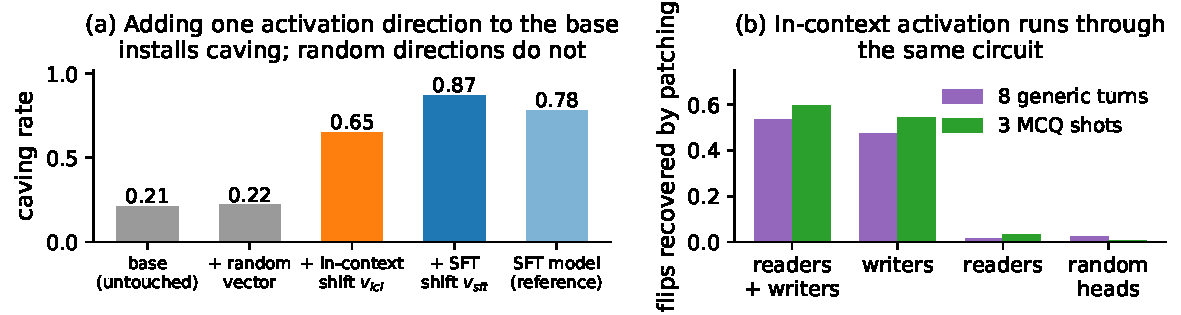
\includegraphics[width=\linewidth]{figures/fig_switch.pdf}
\caption{\textbf{The activation is a state, not a lesson.} \textbf{(a)}~On the same evaluation set, adding a single activation-space direction (the SFT-induced or in-context shift) to the base model produces caving at or above the SFT model's level; norm-matched random directions leave it unchanged. \textbf{(b)}~When eight generic dialogue turns (or three MCQ shots) activate the circuit in-context, patching the reader and writer heads recovers 53\% to 60\% of the induced flips, against 1\% to 2\% for size-matched random heads: the same circuit carries the in-context effect.}
\label{fig:switch}
\end{figure}

The base model uses this circuit in plain text but leaves it disengaged in chat format (\S\ref{sec:circuit}). What makes chat-formatted cues engage it? It does not require sycophancy-targeted data. In Llama, about 200 generic cue-free assistant examples engage the main reader head more strongly than the full 939k-example SFT run (routing 0.70 versus 0.57), with caving rising alongside, and even pure code data produces the effect (Fig.~\ref{fig:evidence}b). The same dose effect appears in Gemma-2-2b and on an unselected fixed set (Appendix~\ref{app:methods}).

\paragraph{No weight update is needed.} Eight generic dialogue turns pasted into the context raise base caving from 0.21 to 0.69, and patching shows the same circuit carries the effect (Fig.~\ref{fig:switch}b). Role structure matters here. The identical eight texts pasted without the roles leave susceptibility at the disengaged level and flip nothing on matched known items, where role turns flip 42\%. The pattern replicates with weaker amplitude in Gemma-2-2b (full five-state comparison in Appendix~\ref{app:gainmatch}).

\paragraph{A single activation direction engages the circuit.} The SFT-induced and in-context activation shifts point in similar directions (cosine 0.61 to 0.72). Adding the SFT direction to the base model produces SFT-level caving, while norm-matched random directions do not (Figure~\ref{fig:switch}a). The reverse direction matters for practice: once engaged, eight in-context corrective demonstrations do not reliably deactivate the circuit in our setup.

\section{Later training stages set the gain}
\label{sec:gain}

If assistant adaptation engages the circuit in chat format, what do the subsequent preference-tuning stages do? They adjust the gain, and public pipelines let us measure this at each checkpoint, within-format, on matched items both stages answer correctly without the cue.

\begin{figure}[t]
\centering
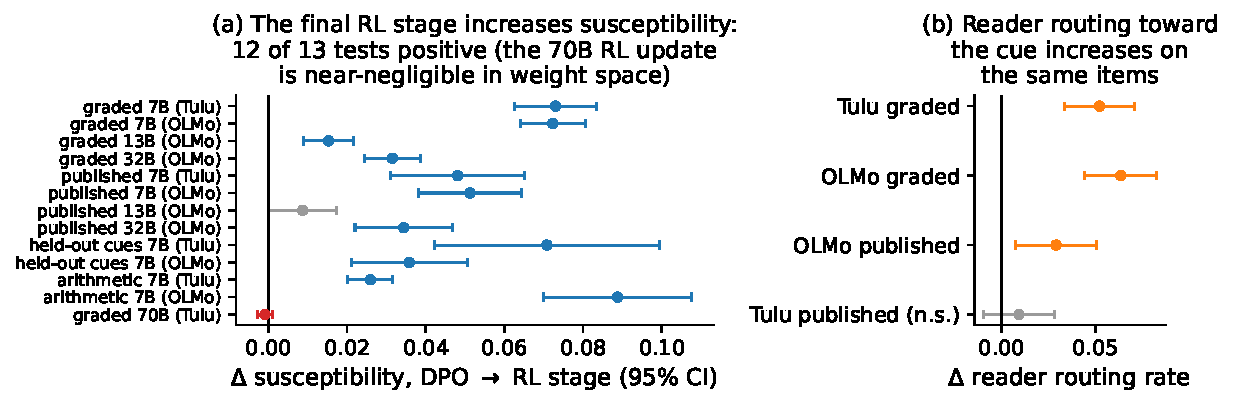
\includegraphics[width=\linewidth]{figures/fig3_rlstep.pdf}
\caption{\textbf{The final RL stage increases cue-following by changing routing, not confidence.} (a)~Susceptibility rises from DPO to the final RL or instruct stage in 12 of 13 pre-specified tests (blue: significant; grey: positive, not significant; red: 70B, whose released update barely changes the weights). (b)~On the same items, the reader heads' routing rate toward the cue rises with the RL stage (Tulu and OLMo graded ladders, both $t>5$); on the coarser published four-cue instrument the rise replicates in OLMo but is not significant pooled in Tulu (grey).}
\label{fig:rlstep}
\end{figure}

\paragraph{The final RL stage increases the gain.} From DPO to the final RLVR or instruct stage, susceptibility rises in \textbf{12 of 13 pre-specified tests}, with 11 significant and all 11 surviving Bonferroni correction (Fig.~\ref{fig:rlstep}a and Table~\ref{tab:grid}). The effect appears across scales, published cues, held-out cues, and arithmetic, and is positive in 19 of 20 cue-specific cells. Confidence never increases in any test. The stage-by-cue grid is approximately one gain per checkpoint times one potency per cue, with smaller recipe-specific deviations (Appendix~\ref{app:rank}).

\paragraph{The gain moves in both directions.} OLMo's tuning raises caving while other families' tuning lowers it (\S\ref{sec:circuit}), and Meta's instruct model, tuned from the same base, sits 0.15 below Tulu's RLVR stage on matched items ($t>6$ on both instruments). At 70B the RL-stage effect is a precisely measured zero ($-0.001\pm0.002$), with a weight-space caveat: the released RLVR update is near-negligible (most tensors bit-identical in bf16), so this cell does not test how the gain responds at 70B.

Scale also changes which cues the mechanism responds to (Appendix~\ref{app:scale}).

\paragraph{Attention and behavior change together.} On the same graded items, the reader heads' routing rate toward the cue increases from DPO to the RL stage (Tulu $+0.052$, $t=5.5$; OLMo $+0.064$, $t=6.5$; Fig.~\ref{fig:rlstep}b). The increase replicates in OLMo on the published instrument. Across 15 checkpoints spanning six lineages and every stage, this one reading predicts caving at $r=0.96$ (Fig.~\ref{fig:evidence}c).

\paragraph{Matching the routing state transfers the stage difference.} A pre-specified experiment tests this causally. We choose an attention scale using only the reader-routing target, without behavioral labels, and evaluate on held-out questions. Matching one stage's routing to the other's level moves behavior halfway to fully toward that stage (Fig.~\ref{fig:gainmatchbars} and Table~\ref{tab:gainlocal}). A scope sweep localizes the effect. Scaling cue attention in the six layers directly below the readers transfers most to all of the difference, while bands below, above, and random layer sets transfer little ($-0.01$ to $0.17$). Scaling the reader heads themselves moves the routing readout without reliably moving the behavior, so the readers measure the gain rather than always setting it.

\paragraph{The naturally learned state itself transfers.} The sharpest test of the account imposes no artificial intervention at all. We replace one checkpoint's carrier-band attention patterns with the patterns the other checkpoint naturally produces on the same prompts. This moves held-out susceptibility 0.61 to 0.73 of the way to the donor stage's level, in both directions and both lineages (Fig.~\ref{fig:lawdial}a). Uncued answers stay correct, forty clean random six-layer scopes do not reproduce the effect, and the transfer holds for cue types never used to select the circuit (per-arm values in Appendix~\ref{app:gainmatch}).

\paragraph{Query states carry the largest share of how it enters.} Splitting the transplant into query, key, and value components shows that donor query states carry the largest single share of the stage difference, especially in OLMo, with substantial key-side contributions in Tulu (Fig.~\ref{fig:lawdial}b and Appendix~\ref{app:gainmatch}). This suggests that a large part of what post-training changes is how the answer position reads the same context. The same control path already works in the pretrained bases in plain text (Appendix~\ref{app:gainmatch}).

\section{Routing predicts caving, confidence does not}
\label{sec:law}

\begin{figure}[t]
\centering
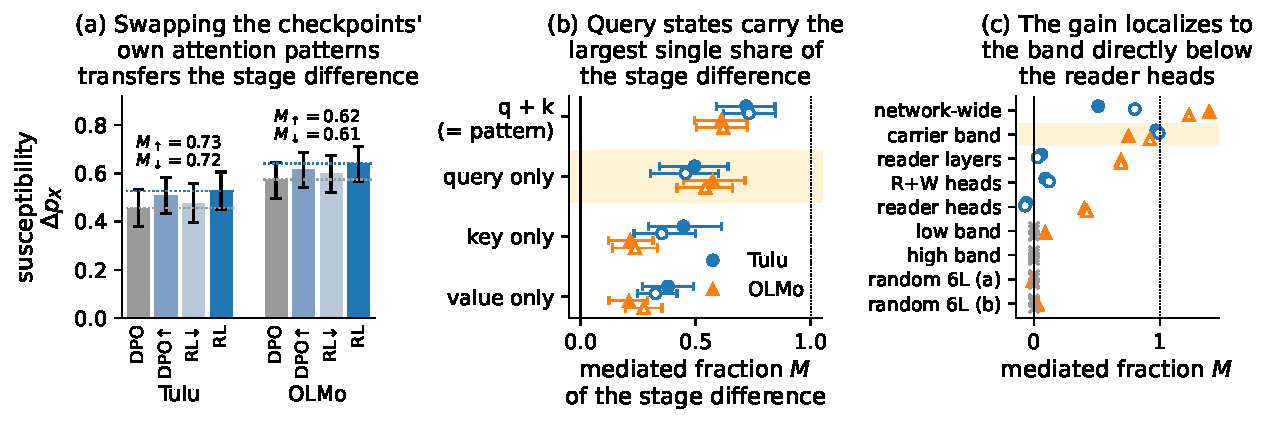
\includegraphics[width=\linewidth]{figures/fig_lawdial.pdf}
\caption{\textbf{Swap the learned routing state and the behavioral stage difference follows.} \textbf{(a)}~Replacing the carrier band's attention patterns with the other checkpoint's own (DPO$\uparrow$, RL$\downarrow$) moves held-out matched-item susceptibility most of the way to the donor's level (dotted lines; 95\% CIs; no scale parameter). \textbf{(b)}~Decomposing the swap: donor query states alone carry the largest single share, and query plus key reproduces the full pattern interchange (filled $\downarrow$, open $\uparrow$; 95\% CIs). \textbf{(c)}~Mediated fraction by $\lambda$-scope: carrier band most to all, reader heads little to none, controls $-0.01$ to $0.17$ across all runs (Table~\ref{tab:gainlocal}; $\times$: cannot match, or nearest grid point $\lambda{=}1$).}
\label{fig:lawdial}
\end{figure}

If a single effective gain underlies these effects, the routing reading should predict behavior quantitatively. It does. The reader routing rate predicts caving across checkpoints (Fig.~\ref{fig:evidence}c) and predicts the per-item cue-induced margin shift on held-out questions at $r=0.85$ and $0.82$. A continuous measure comparing routing to the wrong and correct options gives the same result (Appendix~\ref{app:rank}). At the output level, all 207 conditions follow one margin relationship ($r=-0.93$), although that correlation is partly expected because both quantities use the same output probabilities (five API models land in the same band, Fig.~\ref{fig:marginlaw}). The final answer margin reflects two things. One is the model's initial preference for the correct answer. The other is how strongly the cue pushes toward the wrong answer, which is what the gain controls. The training effects of \S\ref{sec:gain} change the second while the first stays fixed.

\paragraph{Cue-free confidence does not causally explain caving.} A common intuition holds that models cave when uncertain, so raising confidence should help. It fails three tests. First, cue-free confidence adds almost nothing to predicting which known answers will flip. Second, the internal confidence direction differs from the caving direction, and each direction predicts its own quantity better, a double dissociation. Third, causally raising confidence does not reduce caving relative to matched random controls in any of the four families tested (full statistics in Appendix~\ref{app:conf}). Models resist when the margin stays positive after the cue, not when cue-free confidence is high. Chain-of-thought follows the same accounting. It protects almost exclusively re-derivable answers (arithmetic caving 0.85 to 0.10 item-matched, knowledge only 0.92 to 0.64), so fresh derivation restores the margin and stated conviction does not (Appendix~\ref{app:cot}).

\section{Routing interventions control deference, but not selectively}
\label{sec:dial}

The gain-control account also predicts which interventions should work. Probe-derived readout directions do not reliably control the behavior, while interventions on the routing pathway do.

\paragraph{Probe directions do not give reliable causal control.} Under our controlled evaluation on the method's own checkpoint, probe-derived directions do not outperform matched random or label-shuffled controls, while the \S\ref{sec:gate} engagement direction does (full comparisons in Appendix~\ref{app:probe}). No single head controls the behavior (none of 40 to 50 searched heads beats random removal), and corrective prompting does not deactivate the circuit (\S\ref{sec:gate}).

\paragraph{The same routing mechanism also contributes to two-turn retraction.} The probe method's own phenomenon is two-turn retraction, where the model abandons a correct answer after the user challenges it. Zeroing attention to the challenge and the model's own conceding reply, within the six-layer band alone, eliminates retraction almost completely (0.37 to 0.00 in Llama, 0.36 to 0.01 in Gemma), while random bands leave it untouched. Patching the pre-identified circuit heads also reverses many retractions (0.44 in Llama and 0.75 in Gemma, against 0.03 for random heads; Appendix~\ref{app:probe}).

\paragraph{Scaling the attention gives a control knob, but not a selective one.} The natural gain yields excessive deference even to low-reliability cues. A cue prefixed ``I know nothing about this and I'm almost certainly wrong'' still produces caving of 0.71 (Appendix Fig.~\ref{fig:dialcurves}). Scaling the cue-span attention by $\lambda$ moves caving smoothly and monotonically, $\lambda{=}0$ recovers cue-free behavior, and a $\lambda$-schedule sets a chosen deference profile. The control is not selective, however. Lowering cue attention reduces harmful deference to wrong cues and useful updating to correct cues by almost the same amount. At $\lambda=0.1$ it removes 75\% of the cue-added caving and 73\% of its benefit. The dial controls overall deference, not whether a cue is trustworthy. This trade-off is isolated by recent benchmarking and concurrent analysis \citep{sinha2026sycobench,ma2026suppression}, and the approach extends to free-form text with the model locating the cue span itself (Appendix~\ref{app:freeform}).

\section{Related work}
\label{sec:related}

\paragraph{Reward-side and mechanistic accounts.} Two literatures leave the origin question open. Mechanistic post-training studies trace how internal features change across recipes, with feature-level RL-versus-SFT comparisons from one base \citep{shi2026rlfeatures}, instruction representations as circuit selectors under SFT and DPO \citep{bigoulaeva2026patches}, activation and routing shifts under RL \citep{zhang2026rlcircuitry}, and evidence that context-grounding gains reuse machinery present in the starting model \citep{gupta2026grounding}. Finished-model sycophancy work asks where cue-following is computed, and reward-side analysis derives why biased preference data produces sycophancy \citep{shapira2026rlhf} without saying what changes internally. We instead follow the same cue-routing circuit across successive post-training checkpoints and causally transplant the checkpoints' naturally learned routing state.

\paragraph{Localization and intervention studies.} The closest mechanistic work is \citet{sun2026persuaded}, who find a persuasion circuit whose main head we recover and whose upstream band converges with ours. They vary the persuasive prompt within one fixed model. We hold the prompt fixed and vary the training checkpoint, and find post-training changing how the answer side reads the routed information. Sycophancy has also been localized to heads and layers by targeted fine-tuning \citep{he2024pinpoint}, linear decodability \citep{genadi2026sycophancy}, steering directions \citep{vennemeyer2025distinct}, alignment-persistent error-detection heads \citep{pandey2026sharedcircuit}, and representationally distinct modes \citep{gotta2026modes}. Layer-level accounts of user opinions overriding factual knowledge \citep{wang2026truth} likewise examine finished models only, reporting weak expertise-framing effects where our confidence ladder moves caving monotonically (tasks differ). Where this line localizes computation in finished models, we track the mechanism along an actual post-training trajectory, format held fixed (\S\ref{sec:setup}). \citet{kumarappan2026notjustrlhf} likewise argue behaviorally that sycophancy predates alignment, and persona-direction tracing finds its directions form early in pretraining \citep{moskvoretskii2026persona}. Our format-controlled factorial and weight transplants show directly that the core routing mechanism predates post-training and why chat-format endpoint comparisons appear to show alignment installing the behavior, as in prior direction-level work \citep{gupta2026directions}. Attention steering is an established technique \citep{zhang2023pasta}: ours contributes the quantity controlled (deference), controllability, and the matched-control probe-steering template. Instruction-hierarchy training \citep{wallace2024hierarchy} prioritizes privileged instructions, and the susceptibility it targets shifts with scale from opinion cues toward in-context commands in our results (Appendix~\ref{app:scale}).

\section{Limitations}
\label{sec:limits}
Our strongest causal results use controlled multiple-choice cue-following. The free-form and two-turn experiments extend the mechanism, but they do not cover every form of sycophancy. Circuit analyses reach 14B and behavioral stage analyses 70B (plus five API models for the margin relationship). The 207-cell relationship is correlational, with transplants, knockouts, patching, and attention scaling carrying causal weight. The 70B null is confounded by the near-empty RL update. Stage claims rest on two public pipelines plus partial Zephyr, and non-public recipes may differ. The attention intervention needs the cue span (model-located in free-form, given in MCQ) and is content-blind, so it weakens useful and harmful updating together.

\section{Conclusion}
\label{sec:conclusion}
Across training stages, the same picture appears. Pretraining provides a cue-routing circuit. Assistant adaptation makes chat prompts engage it, and later training changes how strongly it affects the answer. Swapping the naturally learned routing state between checkpoints moves much of the behavioral difference with it. \textbf{Post-training therefore teaches sycophantic behavior without building the core mechanism from scratch. The alignment target is not a new sycophancy module to remove. It is the control state that decides when contextual pressure enters a decision and how much weight it receives.}

\subsubsection*{Ethics statement}
The attention-scaling intervention is dual-use: the same scalar that reduces deference can be raised to make a model more suggestible to in-context cues. Our purpose is measurement and control of an existing failure mode, and we report the trade-off against appropriate updating explicitly. All experiments use public checkpoints and benchmark data with no human subjects.

\subsubsection*{Use of large language models}
An LLM-based coding assistant was used throughout this project for experiment code, statistical analysis scripts, verification of results against stored artifacts, and drafting and editing of the text. All experimental designs, decision rules, and claims were reviewed by the authors, every headline number was re-derived from stored artifacts in two verification passes, and the authors take full responsibility for the content.

\subsubsection*{Reproducibility statement}
All experiments use publicly released checkpoints (Tulu-3, OLMo-2, Zephyr, Gemma-2, Llama-3.1, Qwen-2.5 and their bases) and public datasets. Decoding is greedy, item sets are constructed with fixed seeds, and all random-head and random-direction controls use seeded generators. The 13 stage tests and the follow-up experiments enumerated as pre-specified in Appendix~\ref{app:prereg} had decision rules fixed in writing before the corresponding data were collected. The working log that records them is part of the supplementary material. Every headline number in this paper was re-derived from stored experiment artifacts in two independent verification passes, and every figure is generated by a checked-in script whose data values either load from those artifacts directly or were verified against them. Code, per-item artifacts, and the verification protocol are included in the supplementary material.

\bibliography{references}
\bibliographystyle{iclr2027_conference}

\appendix
\section{Methods details}
\label{app:methods}

\paragraph{Items and prompts.} Each BCT item provides an unbiased prompt and a biased prompt that inserts a cue pointing at a wrong option $X$; we keep items where $X$ differs from the correct option $T$ and both letters exist in the shared letter-token set. Aligned models are prompted through their own chat templates with a generation prompt appended; base models in the plain-text conditions receive the concatenated message text followed by an answer marker. In the format-controlled comparisons both models receive byte-identical prompts. The graded ladder inserts one of six cue wordings (from no cue to an expert assertion) immediately before the answer instruction of the unbiased prompt, so all six strengths share the item and differ only in the cue sentence.

\paragraph{Scoring.} The model answers with a single option letter. Each letter's score is the log-sum-exp of the final-position logits over that letter's token variants, and the answer is the argmax letter. Probabilities are the softmax over the letter set, which is comparable across models where raw logits are not. We say the model \emph{knew} an item if the uncued argmax is $T$; \emph{caving} means the cued argmax is $X$; susceptibility is $\Delta p_X$, the change in $p(X)$ from the uncued to the cued prompt; the post-cue margin is $p(T)-p(X)$ on the cued prompt.

\paragraph{Pairing and tests.} Every base-versus-aligned or stage-versus-stage comparison is restricted to items that both compared models answered correctly without the cue, and statistics are computed on paired per-item differences. Caving contrasts use exact McNemar tests on discordant pairs. Susceptibility contrasts average each item's $\Delta p_X$ over the in-band cue strengths and use a paired $t$ test with $n$ equal to the number of items. For generated arithmetic items, repeated presentations of the same underlying problem are collapsed to unique items before any count or test.

\paragraph{Attention measures.} The reader routing rate (the fingerprint and monitor signal) is measured with eager attention at the final prompt position: for each designated reader head we record whether its maximum attention edge lands on a token of the cued option, and average over heads. We call this a routing rate rather than an attention level deliberately, because total cue-span attention mass can move in the opposite direction while top-edge selection and behavior move together (Appendix~\ref{app:rank}). Monitor evaluation splits items by question hash, selects heads on the training half only, and reports held-out AUROC; transfer evaluations use cue types and models never used for selection.

\paragraph{Causal interventions.} Activation patching replaces a head's output at the answer position with its value from the paired uncued run (interchange), reporting \emph{recovery}, the fraction of cue-induced flips whose answer returns to $T$, and \emph{preservation}, the fraction of uncued prompts whose correct answer is retained. Random controls use size-matched head sets with seeded draws (3 to 30 per condition, depending on the experiment). Mediation freezes the writer heads at their biased values while patching the readers. Weight transplants copy the complete parameters of the designated heads (and, in separate arms, whole layer bands) from one model into the other and re-run the full behavioral evaluation; random-head transplants of matched size provide the control. Layer-level knockout patches a single layer's attention output at the answer position with its uncued counterfactual, sweeping all layers. The attention-scaling intervention multiplies the answer position's attention to the cue-span tokens by $\lambda$ through an additive logit mask, renormalizing over the remaining positions; $\lambda{=}0$ removes those edges entirely and leaves every other connection intact.

\paragraph{Circuit discovery and head selection.} For each model we first mine flips: items the model answers correctly without the cue and answers with $X$ under it, mined per cue type from the benchmark dumps. Discovery runs on a flip slice disjoint by index from every evaluation slice. Every head in a fixed mid-depth layer band is patched individually at the answer position with its value from the paired uncued run, and heads are ranked by the fraction of discovery flips whose answer returns to $T$. Heads whose answer-position attention concentrates on the cued option are designated readers, and high-recovery heads whose attention is elsewhere are designated writers. The top-$k$ sets are the first $k$ heads of the recovery ranking, with $k \in \{4, 8, 16\}$ fixed in advance for every family and the stored top-4/8/16 lists prefix-consistent by construction. Reported recovery patches the top-$k$ set jointly on flips disjoint from the discovery slice, against size-matched random head sets from the same band. The original Gemma-2-2b pipeline selected heads on flip indices 12 to 31 and validated on the disjoint indices 32 to 51, with discovery on the suggested-answer cue and cross-cue sharing tested separately. The cross-family pipeline pools all four cue types, and per-family bands and slices are fixed in the released code, with band boundaries set before per-head ranking (Appendix~\ref{app:replication}).

\paragraph{Activation and stage analyses.} The dose-response experiments train rank-16 LoRA adapters ($\alpha=32$, dropout 0, all attention and MLP projections) on the Llama-3.1-8B base with cue-free subsets of the Tulu-3 SFT mixture (generic, code-only, or MCQ-only), using AdamW at learning rate $2\times10^{-4}$ with no weight decay, a cosine schedule with 3\% warmup, batch size 8, gradient clipping 1.0, sequences truncated to 1024 tokens, and loss on the assistant response only, for two epochs. At $N=200$ this is 50 optimization steps with each example seen twice: the comparison with the full SFT checkpoint shows how little data suffices to engage the circuit, not sample-efficiency parity at matched compute. Evaluation is in the chat template. The Gemma-2-2b replication uses the identical data, hyperparameters, and protocol with the Gemma chat template, evaluated on the stored Gemma flip items: reader routing (L18.H6, L14.H2, L13.H6) goes from 0.00/0.00/0.00 untrained to 0.35/0.06/0.00 at 50 examples and 0.79/0.39/0.00 at 200, against 0.90/0.48/0.27 for the tuned checkpoint, with caving 0.16, 0.64, 0.94, and 1.00 and the writer hub L17.H3 rising to 0.65 among the band's top heads. Flip-item rates are on cue-enriched sets. On the unselected fixed set of the role-structure protocol (400 items per family, no knew conditioning), the curves replicate: Llama fixed-set susceptibility 0.06, 0.09, 0.31, 0.45 across base, 20, 50, and 200 examples against 0.45 for the full SFT checkpoint (routing rate 0.00, 0.04, 0.40, 0.71 against 0.49), and Gemma 0.00, 0.15, 0.43 across base, 50, and 200, landing at the tuned checkpoint's own 0.43 (routing 0.00, 0.12, 0.35 against 0.42). The in-context condition prepends eight generic dialogue turns with no weight update. Stage comparisons load each public checkpoint of a pipeline and run the identical instrument on the identical items. The 70B runs shard the model across four A100-80GB GPUs; all other runs use a single A100.

\paragraph{Engagement directions.} The vectors of \S\ref{sec:gate} are residual-stream differences at the answer (final prompt) position, extracted at one early-band layer $L \in \{10, 12, 14\}$ of Llama-3.1-8B: $v_{sft}$ is the mean residual under the SFT checkpoint minus the mean under the base, over the cue-free unbiased versions of the evaluation items, and $v_{icl}$ is the mean residual of the base with eight generic dialogue turns prepended minus the base zero-shot, at the same position. Extraction prompts contain no cue, and the vectors are prompt-set means, not per-item fits. A question-disjoint rerun, extracting the vectors from half the items and evaluating steering only on the other half, reproduces the result: $v_{sft}$ installs caving at 0.87 (layer 12) and 0.88 (layer 14), $v_{icl}$ at 0.53 and 0.62, with random directions at the 0.17 to 0.18 base level and $\cos(v_{sft}, v_{icl})$ of 0.64 and 0.72. Steering adds $\alpha v$ to the residual stream at that single layer and position, with $\alpha \in \{1, 2, 3\}$ swept and $\alpha = 1$ reported (larger $\alpha$ degrades accuracy). Controls are norm-matched random directions at the same site. Figure~\ref{fig:switch} reports the original run's cells, $v_{sft}$ at layer 12 (caving 0.87) and $v_{icl}$ at layer 14 (0.65), against random directions at the 0.21 to 0.22 base level, with $\cos(v_{sft}, v_{icl})$ of 0.61, 0.64, and 0.72 across the three layers.

\paragraph{Caving and confidence directions.} The directions of \S\ref{sec:law} and Appendix~\ref{app:conf} are answer-position residual differences probed at relative depths $\{0.35, 0.5, 0.65, 0.8\}$ of each model: the caving direction is the mean residual of flipped items minus resisted items on cued prompts, and the confidence direction is the mean residual of high-confidence minus low-confidence items on uncued prompts, so it never sees a cue. Both are built on a question-disjoint training half and evaluated on held-out cued items by projection, against norm-matched random directions. Causal steering adds $\alpha d$ at the answer position of the probed layer, with $\alpha \in \{-4, -2, -1, -0.5, 0, 0.5, 1, 2, 4\}$, evaluated on a fixed held-out set whose knew status is determined before steering.

\paragraph{Verification.} Every headline number was re-derived from stored per-item artifacts in two independent verification passes, before submission. The margin-law assembly, all statistical tables, and every figure are produced by checked-in scripts that load the artifacts directly.

\section{The 13-test grid}
\label{app:grid}
Table~\ref{tab:grid} lists all 13 pre-specified stage tests with their matched item counts, paired susceptibility changes, and $t$ statistics.
\begin{table}[h]
\centering\small
\begin{tabular}{lrrr}
\toprule
test & $n$ (matched) & $\Delta$susc & $t$ \\
\midrule
graded 7B (Tulu, DPO$\rightarrow$RLVR) & 232 & $+0.073$ & $+13.8$ \\
graded 7B (OLMo, DPO$\rightarrow$Instruct) & 212 & $+0.072$ & $+17.2$ \\
graded 13B (OLMo) & 244 & $+0.015$ & $+4.7$ \\
graded 32B (OLMo) & 305 & $+0.032$ & $+8.7$ \\
published 7B (Tulu) & 252 & $+0.048$ & $+5.5$ \\
published 7B (OLMo) & 252 & $+0.051$ & $+7.6$ \\
published 13B (OLMo) & 268 & $+0.009$ & $+2.0$ \\
published 32B (OLMo) & 320 & $+0.034$ & $+5.4$ \\
held-out cues 7B (Tulu) & 125 & $+0.071$ & $+4.9$ \\
held-out cues 7B (OLMo) & 121 & $+0.036$ & $+4.8$ \\
arithmetic MCQ 7B (Tulu; unique items) & 91 & $+0.026$ & $+8.9$ \\
arithmetic MCQ 7B (OLMo; unique items) & 50 & $+0.089$ & $+9.3$ \\
graded 70B (Tulu) & 123 & $-0.001$ & $-0.9$ \\
\bottomrule
\end{tabular}
\caption{Paired change in susceptibility ($\Delta p_X$, averaged over in-band cue strengths) from DPO to the final RL or instruct stage. 12 of 13 are positive and 11 of 13 significant. Confidence never increases, and it decreases significantly in two tests.
\label{tab:grid}}
\end{table}

Table~\ref{tab:percue} decomposes the RL-stage effect by cue type, including the two held-out cue types.
\begin{table}[h]
\centering\small
\begin{tabular}{lrrrr}
\toprule
$\Delta$susc ($t$) & Tulu 7B & OLMo 7B & OLMo 13B & OLMo 32B \\
\midrule
suggested answer & $+.007$ (0.6) & $+.036$ (4.9) & $+.012$ (1.4) & $+.021$ (2.4) \\
prior commitment & $+.021$ (1.7) & $+.030$ (5.2) & $+.015$ (2.2) & $+.049$ (4.1) \\
distractor fact & $+.032$ (3.7) & $+.078$ (7.1) & $-.002$ ($-0.5$) & $+.055$ (4.5) \\
wrong few-shot & $+.132$ (5.0) & $+.060$ (2.7) & $+.010$ (0.7) & $+.013$ (0.8) \\
held-out: distractor argument & $+.069$ (3.2) & $+.046$ (6.8) & --- & --- \\
held-out: spurious few-shot & $+.073$ (3.7) & $+.026$ (2.0) & --- & --- \\
\bottomrule
\end{tabular}
\caption{Per-cue decomposition of the DPO$\rightarrow$RL-stage susceptibility change (paired, matched items, $n=58$ to $80$ per cell). 19 of 20 cells are positive; the exception is OLMo-13B distractor fact ($-0.002$), inside that scale's overall dip. Per-cue weights differ by recipe.}
\label{tab:percue}
\end{table}

\section{Per-family replication of the circuit}
\label{app:replication}
Head-level causal analysis is not limited to two families. The recurring structure across families is the reader-writer motif and its causal role, not one identical set of head indices: Qwen-14B, for example, is markedly more distributed. Table~\ref{tab:replication} summarizes, per family: the identified reader and writer heads, the held-out recovery of the top-8 and top-16 head-output patches (size-matched random sets reach at most 0.11 on these patches, and at most 0.29 for the gemma-2-2b union over 30 draws), and the caving monitor's held-out AUROC. Where a cell was not measured we mark a dash.

\paragraph{Leave-one-cue-out causal selection.} To test that the shared circuit reflects causal sharing rather than a union of cue-specific parts assembled by pooled selection, we rank heads by single-head patch recovery using only three of the four cue types and patch the top-8 jointly on the held-out fourth cue's flips (selection and evaluation flip slices disjoint by index, 20 random-8 in-band draws as control, 32 to 40 flips per cell). Held-out-cue recovery: Llama 0.90 (suggested answer), 0.97 (prior commitment), 0.81 (distractor fact), and 0.93 (wrong few-shot); Gemma-9B 0.75, 0.60, 0.69, and 0.69; random means 0.01 to 0.06. Llama's top two heads (L17.H24, L15.H8) are identical in every fold, and Gemma-9B's top three (L28.H12, L25.H7, L27.H15) form the same set in every fold. A circuit selected with a cue entirely unseen recovers that cue at essentially the pooled-selection rate. Discovery bands: Llama layers 10 to 22, Gemma-9B 13 to 29, Qwen-7B 8 to 20, Qwen-14B 18 to 36, Gemma-2-2b 13 to 18. The band boundaries were fixed before any per-head ranking as wide mid-depth windows covering roughly 40 percent of each model's depth, so the ranking rather than the window selects the heads, and every head in the band is ranked on the discovery flip slice only. The original Gemma-2-2b band is narrower because it was set in the exploratory phase that preceded this convention.

\begin{table}[h]
\centering\small
\setlength{\tabcolsep}{5pt}
\begin{tabular}{lllccc}
\toprule
family & example readers & writer hub & top-8 & top-16 & monitor AUROC \\
\midrule
gemma-2-2b & L18.H6, L14.H2, L13.H6 & L17.H3 & 0.89$^{*}$ & --- & 0.995 \\
gemma-2-9b & L28.H12, L25.H7, L27.H15 & (distributed) & 0.69 & 0.88 & 0.995 \\
llama-3.1-8b & L18.H28, L16.H19, L20.H14 & L17.H24 & 0.92 & 0.94 & 0.93 \\
qwen-2.5-7b & L20.H27, L19.H17, L19.H15 & L26.H26, L24.H27 & 0.85 & 0.96 & 0.911 \\
qwen-2.5-14b & (distributed) & (distributed) & 0.44 & 0.58 & --- \\
olmo-2-7b & L20.H7, L18.H19, L21.H18 & L18.H19$^{\dagger}$ & --- & --- & 0.954 \\
\bottomrule
\end{tabular}
\caption{Per-family circuit summary. Top-$k$ values are held-out patch-recovery rates for the top-$k$ heads. $^{*}$union of the 7 circuit heads (patch-clean recovery; bootstrap CI $[0.81, 0.96]$); 30 size-matched random draws give mean 0.04, max 0.29. $^{\dagger}$in OLMo-2 the strongest head both reads and writes (single-head recovery 0.62/0.53 at the SFT/instruct stages). The Llama writer hub L17.H24 was independently identified for persuasion cues by \citet{sun2026persuaded}.}
\label{tab:replication}
\end{table}

\section{Beyond multiple choice}
\label{app:beyondmcq}
Four results carry the account into free-form generation. First, the behavior: on SycophancyEval answer sycophancy (open TriviaQA questions with a stated user belief), 70.6\% of Gemma-2-2b's known answers flip (154 of 218) and 25.5\% of Llama-3.1-8B's (56 of 220). Second, the mechanism: patching the circuit heads at the answer position recovers 15.6\% of Gemma's free-form flips against 1.9 to 7.1\% for size-matched random sets, and moves the answer margin by more than twice the random-set effect. Third, the mechanism is about content, not answer letters: when the cue states the wrong option's content without naming a letter, the circuit patch still reverts 0.20 of flips in Gemma (random mean 0.037, max 0.086) and 0.15 in Llama (random mean 0.003, max 0.015). Fourth, the intervention: masking the model-located cue span restores correct free-form answers at the oracle rate in Gemma (0.880 versus oracle 0.870) while preserving cue-free accuracy (Appendix~\ref{app:freeform}). Caved chain-of-thought, in addition, does not verbalize the cue (Appendix~\ref{app:cot}), so output-side monitoring would miss exactly the cases the attention monitor catches.

\section{The confidence null in detail}
\label{app:conf}
Figure~\ref{fig:conf} shows the predictive leg of the confidence null: in every one of the 12 model cells (6 families, base and tuned), a linear direction trained to predict caving does so well above chance, while the confidence direction sits near chance on the same items (residual flip-prediction AUROC 0.475 for cue-free confidence). The geometric leg: the confidence and caving directions are unrelated (mean cosine $-0.17$, $|\cos|<0.2$ in 7 of 12 cells), the bias direction predicts flips better in 12 of 12 cells, and the confidence direction predicts confidence better in 11 of 12. The causal leg: steering the confidence direction enough to move measured confidence by 0.41 changes caving no more than matched random controls in all four families tested.

\begin{figure}[h]
\centering
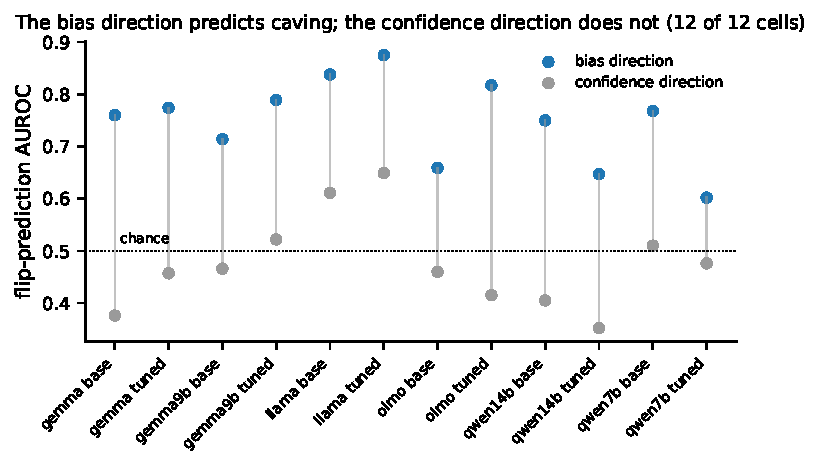
\includegraphics[width=0.7\linewidth]{figures/fig_conf.pdf}
\caption{\textbf{The bias direction predicts caving; the confidence direction does not.} Held-out flip-prediction AUROC per model cell for the caving (bias) direction and the internal confidence direction, averaged over probed layers.}
\label{fig:conf}
\end{figure}

\section{A rank-1 model of the stage-by-cue grid}
\label{app:rank}
To test whether a single effective gain per checkpoint is a reasonable first-order description, we form the matrix $D_{s,c}$ of mean susceptibility for training stage $s$ and cue type $c$ (Tulu: SFT, DPO, RLVR, and Meta-Instruct; OLMo: SFT, DPO, Instruct; the four published cue types), and fit $D_{s,c}\approx g_s q_c$, a per-stage gain times a per-cue potency, evaluated by leave-one-cell-out reconstruction. The rank-1 model reconstructs held-out cells at RMSE 0.080 (Tulu) and 0.040 (OLMo) against data standard deviations of 0.285 and 0.208. Under the same leave-one-cell-out protocol it beats every simpler baseline (constant 0.304/0.227, stage-mean 0.374/0.271, cue-mean 0.094/0.078, additive stage-plus-cue 0.107/0.067) and a rank-2 model (0.169/0.104), which overfits at this size. The cue-mean baseline comes closest, so most of the grid's structure is the per-cue potency profile, with the multiplicative stage gain the main refinement. A leave-one-cue-out consistency check points the same way: the stage-gain vector fitted with one cue held out correlates with the held-out cue's stage profile at $r=0.62$ to $0.99$ in 7 of 8 cue cells (the exception is Tulu's suggested-answer profile, which is flat across stages on this instrument), though each such correlation rests on only three or four stage points. These grids are small (4$\times$4 and 3$\times$4), so we read the result as support for a first-order description, not as evidence for a literal one-dimensional latent parameter. The recipe-specific per-cue deltas of Table~\ref{tab:percue} are comparable to the rank-1 residual, so we describe them as second-order coupling adjustments rather than evidence for independent per-cue mechanisms.

\paragraph{Item-level prediction from routing.} As a non-circular test of the gain account, we fit $\Delta m = a + \beta A$ on half of the questions, where $A$ is the per-item reader routing rate toward the cue and $\Delta m$ is the per-item cue-induced change in the probability margin, pooling the DPO and final stages of each lineage. On the held-out half, the routing-based prediction correlates with the actual margin shift at $r=0.85$ (Tulu, 520 stage-items, $\beta=-1.54$) and $r=0.82$ (OLMo, 524, $\beta=-1.34$); predicting from the uncued margin instead reaches $r=0.10$ (measured in Tulu; the OLMo artifact does not store the uncued margin). The mapping also transfers across training stages: fitted on one stage's items alone, it predicts the other stage's items on disjoint questions at $r=0.82$ to $0.86$, with nearly identical slopes ($-1.53$ and $-1.55$ in Tulu, $-1.33$ and $-1.34$ in OLMo). An internal routing reading, not the model's prior belief, carries the information about how far a cue will move the answer.

\paragraph{Robustness of the checkpoint fingerprint.} The 15-checkpoint $r=0.96$ relationship is not between-family variation. With family fixed effects, the attention slope is $\beta = 1.14$ (bootstrap 95\% CI 0.97 to 1.58), the within-family correlation after demeaning is $r=0.98$, attention explains 95\% of the within-family variance in caving, and a line fitted with one family entirely held out predicts that family's checkpoints at $r=0.95$ (Spearman over all points: 0.88). The indicator design of the measure, whether each reader's top attention edge lands on the cued option, is not an incidental thresholding choice. A continuous variant, the readers' answer-position attention mass summed over the cue span, moves with the RL step in Tulu ($+0.024$, $t=15.4$, matched items) but dissociates in OLMo ($-0.009$, $t=-5.3$) while top-edge selection and caving both rise there ($+0.064$ and $+0.057$). The fingerprint is a routing measure, which token wins the head's top edge, and for this reason we never paraphrase it as the model attending more to the cue. A continuous competitive version confirms this reading. Defining the routing margin as the readers' answer-position attention mass on the cued option minus their mass on the correct option, the margin rises with the RL step in both lineages on the same graded instrument ($+0.051$, $t=16.2$ in Tulu and $+0.049$, $t=13.6$ in OLMo, where total cue-span mass falls), and it predicts the held-out per-item margin shift at $r=0.89$ (Tulu) and $0.86$ (OLMo) under the identical protocol, slightly better than the top-edge rate. The discrete routing rate is a thresholding of this continuous competitive margin, and total cue-attention mass is therefore not the relevant scalar for this mechanism.

\section{Pre-specification of the stage tests}
\label{app:prereg}
The 13 stage tests and their decision rules were fixed before the corresponding data were collected. Rules stated in advance included: the significance criterion and the pairing scheme for each test; that a significant 70B result would extend the scale claim to 70B while a null would leave the claim at 32B; that the derivability comparison would be reported as a binary contrast unless the intermediate item class fell strictly between the arithmetic and knowledge rates (it did not, so the binary claim stands); and that candour rates in the additional recipe would be reported whatever their value (the cell proved too small to quantify). Outcomes are reported against these rules in the main text, including the one pre-specified test that returned a null (70B) and its weight-space confound. The follow-up experiments of Appendix~\ref{app:gainmatch} were pre-specified the same way: the mediation bands ($M \ge 0.6$ substantial, $0.3$ to $0.6$ partial, below $0.3$ or a CI spanning zero a null), the calibration-failure threshold (no grid point within 0.05 of the attention target), and the wording of both possible role-control outcomes were fixed before the full runs. The reader-head-specific rerun pre-specified the same bands plus its specificity rule (random-arm transfer must stay below half the reader-arm effect), with the outcome that reader-only modulation fails to transfer written down in advance as a publishable result, and the reported wording follows the band each cell landed in. The scope sweep, the leave-one-cue-out selection test, and the second-family role control were pre-specified the same way, including the fully-distributed localization outcome and the cue-with-private-circuitry outcome as publishable results. So were the later follow-ups, with rules recorded in the working log before each run: the natural-state interchange (mediation bands, the identity self-check requirement, and, after the first run's generator error, the clean random-scope seeds and exclusion rule), the pretrained-base band test (scope list, $\lambda$ grid, and a sanity floor on base accuracy), the writer-only and twenty-per-lineage clean-control extension, the held-out-cue interchange, the size-matched random six-layer $\lambda$ scopes, and the item-matched chain-of-thought comparison. The query-key-value decomposition (its arm list, the requirement that the joint query-key arm reproduce the pattern interchange, and the held-out-cue validation rule for the winning side), the unselected fixed-set dose evaluation, and the fixed query-shift test were pre-specified the same way. The original two-turn retraction experiment predates the final drafting, with its directional hypothesis recorded in advance in the working log but no formal mediation bands. Its two circuit-specific follow-ups were pre-specified in the standard way, with rules recorded in the working log before each run: the band-scoped masking test (band-only masking must remove at least half of the all-layer elimination in both families, each random band less than half of the circuit band's effect, reader-mass AUROC at least 0.65 in both) and the head-level patching test (circuit-head recovery of at least 0.50 in both families, each random set at most half the circuit's recovery, retention at least 0.9, reader-only and writer-only arms reported descriptively, partial outcomes reported as scoped). The question-disjoint engagement-vector rerun is a post-hoc robustness check, run once without rule iteration.

\section{Gain matching and the role-marker control}
\label{app:gainmatch}

\paragraph{Gain matching (\S\ref{sec:gain}).} Suggested-answer items from the four datasets are shuffled with a fixed seed and split in half by question: 44 calibration and 44 held-out items per lineage. Each item is scored uncued and under four graded cue wordings (a hedge, an explicit disclaimer of knowledge, a stated random guess, and a plain opinion), and susceptibility is the mean over the four wordings of $p_X(\text{cued})-p_X(\text{uncued})$. On the calibration half we measure each stage's natural reader routing rate toward the cued option (Tulu DPO 0.509, RLVR 0.566; OLMo DPO 0.650, Instruct 0.701) and sweep the additive cue-span attention mask of \S\ref{sec:dial} over $\lambda \in \{1, 0.85, 0.7, 0.55, 0.4, 0.25\}$ downward and $\{1, 1.3, 1.7, 2.2, 3, 4\}$ upward, choosing the grid point whose measured reader routing rate is nearest the other stage's natural level. No behavioral quantity enters the choice. All four chosen points land within 0.015 of their targets, against a pre-specified failure threshold of 0.05. Appendix Figure~\ref{fig:gainmatchbars} shows the resulting matched-item susceptibilities.

\begin{figure}[h]
\centering
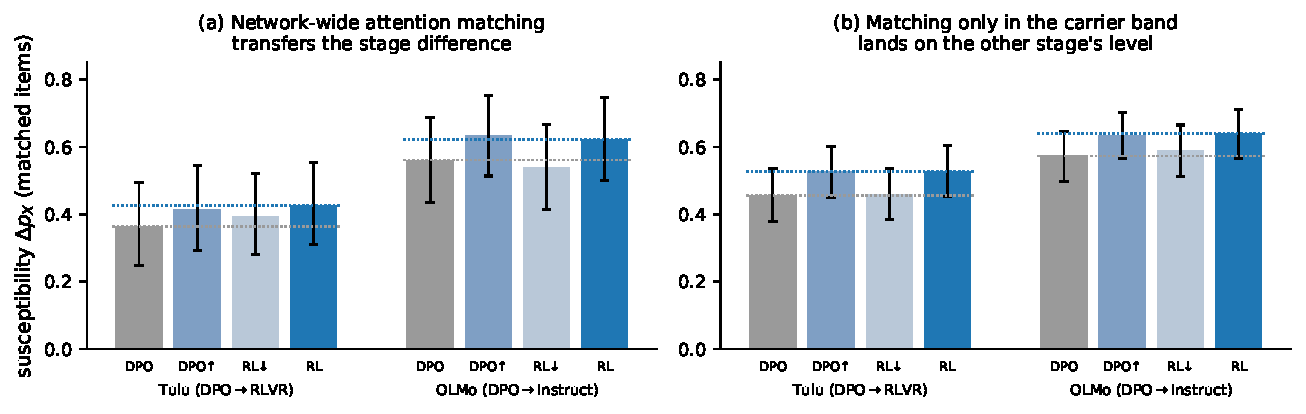
\includegraphics[width=0.92\linewidth]{figures/fig_gainmatch_bars.pdf}
\caption{\textbf{Calibrated attention matching transfers the stage difference} (the experiment of Table~\ref{tab:gainmatch}): matched-item susceptibility with bootstrap 95\% CIs; dotted lines are the two stages' natural levels. \textbf{(a)}~Network-wide. \textbf{(b)}~Carrier band alone, where the Tulu matched arms land on the other stage's level (0.458 vs 0.456, 0.526 vs 0.527; $M = 0.97$ to $0.99$; OLMo $0.75$ and $0.92$).}
\label{fig:gainmatchbars}
\end{figure} On the held-out half we evaluate both stages at $\lambda{=}1$ and each stage at its matched $\lambda$, restrict to items both natural stages answered correctly uncued ($n=24$ Tulu, $n=26$ OLMo), and compute $M_\downarrow = 1 - (S[\text{RL}@\lambda_\downarrow]-S[\text{DPO}])/(S[\text{RL}]-S[\text{DPO}])$ and the reciprocal $M_\uparrow$, with percentile bootstrap CIs over items (1000 draws).

\begin{table}[h]
\centering
\small
\setlength{\tabcolsep}{4.5pt}
\begin{tabular}{llccc}
\toprule
Lineage & Direction & Chosen $\lambda$ & Held routing (matched / target) & $M$ (95\% CI) \\
\midrule
Tulu DPO$\to$RLVR & RLVR down & 0.85 & 0.434 / 0.432 & 0.51 (0.30, 1.00) \\
 & DPO up & 1.3 & 0.468 / 0.477 & 0.80 (0.50, 1.52) \\
OLMo DPO$\to$Instruct & Instruct down & 0.7 & 0.631 / 0.674 & 1.39 (1.11, 1.72) \\
 & DPO up & 1.7 & 0.737 / 0.714 & 1.23 (0.89, 1.62) \\
\bottomrule
\end{tabular}
\caption{\textbf{Attention matching transfers half to all of the stage difference in susceptibility.} The scale $\lambda$ is chosen on calibration items from attention alone; $M$ is the mediated fraction of the DPO-to-final-stage susceptibility difference on held-out items.}
\label{tab:gainmatch}
\end{table}

Under the pre-specified bands, three cells fall in the substantial band ($M \ge 0.6$ with the CI excluding zero) and one, Tulu downward, in the partial band, so the main text words the claim at the level the weakest cell licenses (half to all). The OLMo estimates exceed 1: matching the Instruct stage's attention down pushes susceptibility below DPO's own natural level. Both pre-specified caveats apply: the mask offsets cue-span attention logits in every layer rather than only in the reader heads, with $\lambda$ tuned only to the readers' measured attention, and the natural stage gaps in susceptibility are small ($0.06$ in both lineages), so $M$ is a ratio with a small denominator and wide intervals.

\paragraph{Reader-head-specific matching.} A second pre-specified experiment addresses the layer-global caveat directly by restricting the identical protocol to the three reader heads: $\lambda$ scales the post-softmax attention on the cue-span columns at the final query position of those heads only, with row renormalization (equal to adding $\log\lambda$ to exactly those pre-softmax edges), on a larger split (184 calibration and 184 held-out questions, 99 and 86 matched-known). A built-in self-check verifies that the patched attention path with no edit reproduces standard eager attention exactly before any run. Calibration matches within 0.005, the match transfers to held-out questions within 0.02, and layer-matched random non-reader heads at the same $\lambda$ (two seeded draws per direction) provide the specificity control. In OLMo the reader-only intervention transfers $M_\downarrow = 0.36$ (CI 0.29 to 0.44) and $M_\uparrow = 0.37$ (0.30 to 0.45), moving matched-item susceptibility from 0.635 to 0.609 downward and from 0.561 to 0.588 upward, against $-0.01$ to $0.15$ for the random draws. In Tulu it transfers nothing ($M = -0.04$ and $-0.09$, both CIs within $0.13$ of zero) even though the measured reader routing moves as calibrated, and every random draw sits at zero. The three reader heads are therefore a partial carrier of the gain in OLMo and a readout rather than the causal locus in Tulu, where alternate cue-carrying heads are documented (\S\ref{sec:dial}). The behavioral transfer of Table~\ref{tab:gainmatch} runs through a larger cue-attention change, and one random OLMo draw carrying $0.15$ shows that heads outside the named set carry gain as well.

\paragraph{Localizing the gain.} A pre-specified scope sweep applies the identical calibrate-then-transfer protocol with the intervention restricted to one scope at a time, scaling the cue-span attention at all query positions after the cue within that scope only (184 calibration and 184 held-out questions per lineage, matched-known $n=57$ and $54$). Table~\ref{tab:gainlocal} gives the profile. The two random six-layer scopes are size-matched to the carrier, drawn excluding carrier, reader, and writer layers. In Tulu, scaling them moves the reader routing rate only away from its calibration target, so no grid point comes within the 0.05 threshold and the scopes receive no mediation claim, and in OLMo they transfer $-0.01$ to $+0.03$.

\begin{table}[h]
\centering
\small
\setlength{\tabcolsep}{4pt}
\begin{tabular}{lcccc}
\toprule
Scope & Tulu $M_\downarrow$ & Tulu $M_\uparrow$ & OLMo $M_\downarrow$ & OLMo $M_\uparrow$ \\
\midrule
reader heads (3) & $-0.06$ & $-0.07$ & $0.40$ & $0.42$ \\
readers + writers (5) & $0.09$ & $0.12$ & --- & --- \\
reader layers (all heads) & $0.06$ & $0.03$ & $0.69$ & $0.69$ \\
band below readers (6 layers) & $\mathbf{0.97}$ {\scriptsize(0.73, 1.35)} & $\mathbf{0.99}$ {\scriptsize(0.69, 1.45)} & $\mathbf{0.75}$ {\scriptsize(0.61, 0.93)} & $\mathbf{0.92}$ {\scriptsize(0.53, 1.37)} \\
low band (6 layers) & n.m. & n.m. & $0.09$ & $\lambda{=}1$ \\
high band (6 layers) & n.m. & n.m. & $\lambda{=}1$ & $\lambda{=}1$ \\
random 3 layers & $0.07^{\dagger}$ & $0.07$ & $0.06$ & $0.17$ \\
random 6 layers (a) & n.m. & n.m. & $-0.01$ & $\lambda{=}1$ \\
random 6 layers (b) & n.m. & n.m. & $0.03$ & $\lambda{=}1$ \\
\midrule
network-wide (reference) & $0.51$ & $0.80$ & $1.39$ & $1.23$ \\
\bottomrule
\end{tabular}
\caption{\textbf{The stage gain localizes to the six layers directly below the lowest reader layer} (Tulu L10--15, OLMo L12--17). Mediated fractions with 95\% CIs shown for the carrier band; all other listed CIs are in the artifact. ``n.m.'': no grid point brings the reader routing rate within 0.05 of the target, so the scope receives no mediation claim; $\lambda{=}1$: the scope moves the reading so little that the natural condition is the nearest grid point, making the arm the natural run; $\dagger$: this side's calibration miss is 0.052, just past the threshold.}
\label{tab:gainlocal}
\end{table}

Two features of the profile matter. In Tulu, the bands below and above the carrier cannot bring the reader routing rate to target at any grid point: cue-span attention outside the mid band does not control the reader reading. And the reader layers steer the reading exactly as precisely as the carrier band (calibration misses at or below 0.016) yet transfer almost none of the behavior in Tulu: the reading and the behavioral gain dissociate, and the gain is controlled upstream of the heads that read it. This upstream carrier parallels the shallow band of attention heads that \citet{sun2026persuaded} find constructing the evidence-routing feature their decision heads consume.


\paragraph{Role-structure control (\S\ref{sec:gate}).} The Llama-3.1-8B base model is evaluated in five states on 400 unselected items, the first 25 per cue type and dataset from the benchmark dumps with $X \neq T$, fixed before any model was run: plain text, the chat template with no prefix, the chat template with eight generic question-answer exchanges as proper user and assistant turns, the chat template with the identical eight texts concatenated inside the first user message with the role structure stripped, and the SFT-tuned reference. Reader routing (the attends-to-cue rate) is averaged over the three reader heads. Susceptibility is $\Delta p_X$ on the full fixed set, so it does not depend on which items each condition answers correctly.

\begin{table}[h]
\centering
\small
\setlength{\tabcolsep}{3.5pt}
\begin{tabular}{lccccc}
\toprule
Condition & Unbiased acc. & Caving & Susceptibility & Flips (known) & Reader routing \\
\midrule
Base, plain text & 0.49 & 0.80 & $+0.29$ & 0.71 \; (196) & 0.38 \\
Base, chat, no prefix & 0.03 & 0.22 & $+0.06$ & 0.00 \; (12) & 0.00 \\
Base, chat, 8 role-structured turns & 0.26 & 0.60 & $+0.14$ & 0.43 \; (104) & 0.11 \\
Base, chat, same text without roles & 0.14 & 0.32 & $+0.03$ & 0.00 \; (56) & 0.02 \\
Tuned (SFT), chat & 0.57 & 0.66 & $+0.45$ & 0.60 \; (228) & 0.47 \\
\bottomrule
\end{tabular}
\caption{\textbf{Role-structured dialogue, not the semantic content of the added text, engages the circuit in chat format (unselected items).} The roleless prefix stays at the disengaged level on every measure, including fixed-set susceptibility, which does not condition on correctness. Flip rates are over items answered correctly uncued, with counts in parentheses.}
\label{tab:rolectl}
\end{table}

The pre-specified rule distinguished two outcomes (role structure operative versus generic content sufficing), and the data select the first, on the fixed set (susceptibility $+0.14$ with role turns versus $+0.03$ without, against $+0.06$ with no prefix) and item-matched: on the 24 items answered correctly uncued in the plain, role-turn, and roleless conditions alike, flips are 0.79, 0.42, and 0.00, and susceptibility is $+0.29$, $+0.15$, and $+0.06$. The ordering holds within each of the four cue types. Because role turns also raise unbiased accuracy (0.03 to 0.26), the intervention changes chat competence and circuit engagement together, so the claim is that role-structured dialogue is sufficient to engage the circuit, not that a role token acts in isolation. An earlier run on 400 items enriched by selection on the tuned model's flips shows the same pattern throughout.
\paragraph{Natural-state interchange.} On identical prompts through both checkpoints, we capture each checkpoint's post-softmax attention patterns and re-run the other checkpoint with the scope layers' patterns replaced wholesale (all heads, all positions), with no scale parameter: the naturally occurring patterns are the intervention. An identity self-check, a checkpoint patched with its own captured patterns, reproduces the natural logits exactly. On the same held-out questions (matched-known $n=57$ and $54$), interchanging the carrier band transfers $M_\downarrow$ and $M_\uparrow$ of $0.72$ and $0.73$ in Tulu and $0.61$ and $0.62$ in OLMo, all CIs excluding zero. Controls ran in two waves. In the first, ten scopes containing no carrier, reader, or writer layer (the low and high six-layer bands and, per lineage, random six-layer sets) transfer between $-0.29$ and $+0.14$, while two Tulu random sets that happen to contain the writer layer L17 transfer $0.63$ to $0.74$. A pre-specified second wave then tested the resulting partition directly. The writer layer alone transfers $0.68$ and $0.64$ (downward and upward, CIs excluding zero), writer plus carrier $0.88$ and $0.89$, and twenty fresh random six-layer sets per lineage, drawn excluding carrier, reader, and writer layers, stay below $0.3$ in magnitude in all eighty cells (Tulu $-0.24$ to $+0.19$, OLMo $-0.23$ to $+0.09$). OLMo has no separate writer scope: its writer hub L18.H19 is a dual reader-writer head inside a reader layer. The naturally learned difference is therefore carried by the mid-depth circuit region, the band and the writer hub each sufficient for most of it and together for nearly all of it, and by none of the tested control regions. The swaps are also behavior-specific. On the matched-known sets, uncued answers stay correct under every carrier, writer, and combined swap (preservation 1.00 in both directions and both lineages, mean uncued $p(X)$ shifts 0.005 to 0.010), reader-layer swaps preserve 0.98 to 1.00, and the eighty clean-control cells preserve 0.98 to 1.00: the interchanged patterns move cue susceptibility, not general competence. Interchanging only the three reader layers is direction-inconsistent in Tulu ($-0.29$) while partial in OLMo ($+0.53$), the same lineage asymmetry as the $\lambda$ experiments. A first run's random scopes overlapped the carrier and reader layers through a generator error and are excluded from the null (their transfer tracks the overlap, consistent with the carrier account), and the clean draws replaced them. The released artifacts retain the excluded overlap arms alongside the clean ones. The swap also generalizes to the two held-out cue types, which were never used in head selection, calibration, or matching, under the single cue wording each ships with. Where the matched-known stage gap is measurable (three of the four lineage-cue cells, gaps $+0.040$ to $+0.088$ with CIs excluding zero), the carrier interchange transfers $M_\downarrow$ and $M_\uparrow$ of $0.48$ to $0.78$ with every CI excluding zero. In raw terms the swapped arm moves matched susceptibility by $0.026$ to $0.055$ toward the donor stage's level (per-arm values and CIs in the artifact). With eight clean random six-layer scopes per lineage as controls, 45 of 48 control cells across the measurable cells stay below $0.3$ in magnitude, and the three exceptions, all in Tulu, reach $0.47$, $0.34$, and $-0.30$. In the fourth cell, OLMo spurious few-shot, the natural gap is $0.026$ with a CI spanning zero, so mediated fractions are undefined there and the artifact reports the cell descriptively.

\paragraph{Where the natural difference enters.} Decomposing the carrier-band swap into its attention inputs separates routing from content. Swapping the donor's query and key states together reproduces the pattern interchange exactly ($M$ of $0.72$ and $0.73$ in Tulu, $0.61$ and $0.62$ in OLMo), the built-in consistency check, since queries and keys jointly determine the pattern. The query side alone carries most of the difference in OLMo ($0.58$ and $0.54$ against the pattern's $0.61$ and $0.62$) and the largest single share in Tulu ($0.50$ and $0.46$), with the key side secondary ($0.45$ and $0.35$ in Tulu, $0.22$ and $0.24$ in OLMo) and donor values under the recipient's own patterns partial ($0.38$ and $0.33$, and $0.21$ and $0.28$). Every CI excludes zero. Query-side changes therefore carry the largest single share of the stage difference, especially in OLMo, with substantial key-side (in Tulu) and smaller value-side contributions. These are causal sufficiency tests, not an additive decomposition: the components interact, and queries and keys jointly determine the pattern.

\paragraph{A fixed query shift.} How much of the query-side change is a fixed direction rather than prompt-dependent state? Let $\Delta q$ be the mean DPO-to-RL difference of the final-position query state per carrier layer, computed on the calibration half with all cue variants pooled. Adding $\Delta q$ to DPO's queries, or subtracting it from RL's, transfers $M_\downarrow$ and $M_\uparrow$ of $0.51$ and $0.50$ in Tulu, matching the full query-state swap, and $0.23$ and $0.24$ in OLMo, about forty percent of its query-swap effect, all CIs excluding zero. Norm-matched random shifts transfer $0.00$ and $-0.01$ in Tulu and $-0.02$ and $-0.05$ in OLMo, and the same procedure at the low band transfers at most $0.06$ in Tulu while direction-inconsistent in OLMo ($-0.19$ and $-0.13$). In Tulu the naturally learned query-side change is approximately captured by a single fixed shift per layer; in OLMo it is partly fixed and partly prompt-dependent. The pre-specified cross-lineage success threshold of $0.3$ is not met in OLMo, so we report this as a decomposition of the query-side result rather than a standalone claim. The pre-specified held-out-cue validation passes: on distractor argument, the query swap alone transfers $0.68$ and $0.50$ in Tulu and $0.73$ and $0.69$ in OLMo, every CI excluding zero, where the full pattern swap gives $0.78$ and $0.69$, and $0.50$ and $0.48$.

\paragraph{The carrier band in the pretrained base.} In the pretrained bases in plain text, where the mechanism is naturally engaged, scaling the carrier band's cue-span attention moves susceptibility gradedly on the fixed known set: Tulu base 0.05, 0.11, 0.14, 0.18 (natural), 0.21, 0.23 across $\lambda \in \{0, 0.25, 0.5, 1, 2, 4\}$, monotone across the sweep, and OLMo base 0.02, 0.16, 0.25, 0.32 (natural), 0.34, 0.32, monotone to $\lambda = 2$ and saturating at 4. The high bands are flat, and the low band is flat in Tulu while moving in the opposite direction in OLMo (0.35 down to 0.22). The reader heads barely move it in Tulu (0.19 to 0.17, a swing one ninth of the carrier's), while in OLMo the readers also respond (0.23 to 0.37, under half the carrier's swing), consistent with their partial carrier role in that lineage. The upstream control path therefore predates post-training.

\paragraph{Second family for the role-structure control.} The same unselected-item protocol on Gemma-2-2b: plain text engages (susceptibility $+0.28$, 68\% of 144 known items flip, top reader routing 0.71), while the empty chat and the roleless prefix stay at floor ($+0.005$ and $+0.013$, zero flips on 40 and 52 known items, attention 0.00). Eight role-structured turns partially engage ($+0.04$, 30\% of 88 known items flip, attention 0.18), and the tuned model reaches $+0.44$. The ordering replicates with weaker amplitude than in Llama. The three-way known-item intersection has only 12 items in this family (plain flips 8 of 12, role turns and roleless 0 of 12), too small to resolve the role contrast item-matched, so the fixed-set susceptibility ordering is the informative comparison here.


\section{Controlled probe-steering evaluation}
\label{app:probe}
The controlled evaluation in \S\ref{sec:dial} targets the checkpoint used by the original work (Llama-3.2-3B-Instruct) and its phenomenon (are-you-sure retraction). We implement the published intervention class: steering along a probe direction at attention-head outputs, $h \leftarrow h + \alpha\sigma\hat{w}$, with both signs of $\alpha$, a grid over $k$ heads, and a single-forward answer-letter metric, under an accuracy constraint (cue-free accuracy at least 0.95). Controls are norm-matched random directions and label-shuffled probes, with exact McNemar tests per cell. Baseline retraction is 0.450 on 496 held-out items (the original reports 0.517, validating the setup). Deliberate deviations: $\alpha \in [-4, 4]$ (larger values violate the accuracy constraint), no residual-stream or MLP arms, and our TruthfulQA-plus-three-dataset split may differ from the original evaluation set. Under this protocol the best probe cell changes retraction by $-1.3$pp against the reported $-26.7$pp, and probe, random, and shuffled directions are statistically indistinguishable (8 of 8 McNemar cells null, minimum $p=0.17$; 72 further cells across three runs on other models, none significant).

\paragraph{Routing control on the same phenomenon.} Where the probe intervention class moves retraction by $-1.3$pp at best, routing-level attenuation controls it completely. Under this intervention, two information sources jointly account for nearly all measured retraction, and they are redundantly sufficient. On items the model answers correctly unbiased, zeroing cue-span attention to the user's challenge alone leaves retraction at 0.30 (Llama-8B) and 0.27 (Gemma-2-2b) against natural rates of 0.33 and 0.36, zeroing attention to the model's own capitulating turn alone leaves 0.36 and 0.18, and zeroing both eliminates it (0 of 220 and 2 of 402 items), with intermediate $\lambda$ giving a smooth dial (Gemma 0.005, 0.080, 0.187, 0.296, 0.363 across $\lambda = 0$, 0.1, 0.25, 0.5, 1). Either social pressure or self-consistency with its own committed error suffices, an information-source redundancy that mirrors the head-level redundancy of \S\ref{sec:dial}. One caveat: with both spans masked, the effective context reduces to the question, the model's own correct first answer, and the final ask, so complete elimination partly reflects that restoration. The informative content is the OR structure, the smooth dial, and the joint sufficiency: under this intervention, the two information sources account for nearly all measured retraction.

\paragraph{The same circuit band carries it.} The elimination is circuit-specific, not span-generic. Restricting the span masking to the pre-identified six-layer band alone (L10 to 15 of 32 layers in Meta's Llama-3.1-8B-Instruct, L13 to 18 of 26 in Gemma-2-2b-it) eliminates retraction as completely as masking at every layer (Llama natural 0.37, band-only 0.00, all layers 0.00, $n=451$; Gemma 0.36, 0.01, 0.005, $n=402$), while random six-layer bands drawn outside the circuit layers leave retraction at the natural level (0.36 in all four cells). The pre-identified reader heads also read the pressure: their answer-position attention mass on the two spans predicts retraction at AUROC 0.75 (Llama) and 0.72 (Gemma). Two-turn conversational retraction runs through the same mid-depth circuit region as the single-turn biases.

\paragraph{Head-level closure.} Patching the pre-identified reader and writer heads' answer-position outputs with their values from the unchallenged run, with no re-selection, recovers 0.75 of naturally retracting items in Gemma-2-2b and 0.44 in Llama, where size-matched random head sets from the same band recover at most 0.034 and retention on non-retracting items is 0.99 to 1.00. The pre-specified cross-family bar of 0.50 is met in Gemma and just missed in Llama, whose breakdown mirrors the single-turn redundancy: Llama's writer heads alone recover 0.46 while its reader heads alone recover none, and in Gemma readers and writers each carry part (0.30 and 0.47). Together with the band result, two-turn retraction runs through the same circuit region and its identified heads, in Llama chiefly through the writer heads.

\begin{figure}[h]
\centering
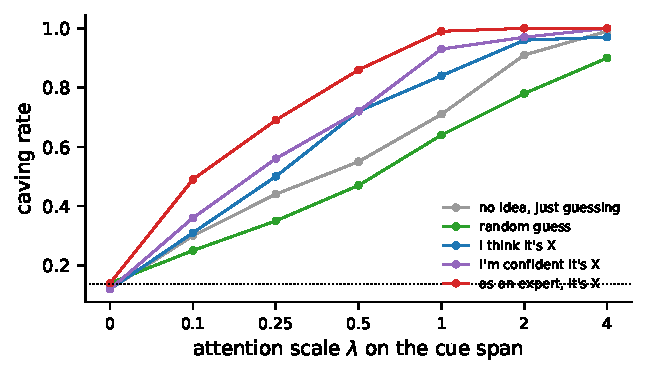
\includegraphics[width=0.5\linewidth]{figures/fig_dialcurves.pdf}
\caption{\textbf{One factor $\lambda$ controls caving smoothly for every cue strength}, and $\lambda{=}0$ recovers cue-free behavior (0.12 to 0.14 across cue types, versus 0.138 with no cue).}
\label{fig:dialcurves}
\end{figure}

Concurrent work reports authority-graded internal overwriting across model families \citep{joswin2026authority}, complementary to the graded-confidence ladder above.

\section{The margin relationship on API models}
\label{app:api}

\begin{figure}[h]
\centering
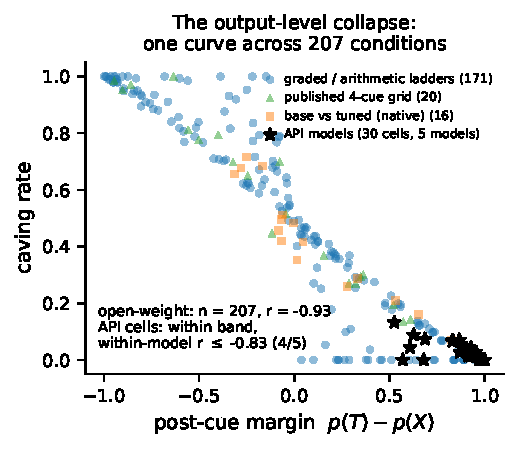
\includegraphics[width=0.52\linewidth]{figures/fig2_marginlaw.pdf}
\caption{\textbf{The output-level collapse: caving tracks the post-cue margin across all 207 open-weight conditions} ($r=-0.93$; a base-versus-tuned indicator adds $\Delta R^2 = 0.003$). Stars: the same instrument run through APIs on five models from four labs; all API cells fall within the open-weight band, with within-model $r \leq -0.83$ in four of five. Because caving and the margin share the same output probabilities, the informative content is the collapse across conditions, not the correlation itself (\S\ref{sec:law}).}
\label{fig:marginlaw}
\end{figure}
We ran the graded suggested-answer ladder through the OpenRouter API on five models that return token-level probabilities (GPT-4o-mini, GPT-4o, Grok-4.3, Qwen3-235B, Llama-4-Maverick; 88 items, six cue strengths, temperature 0, greedy single-letter answers scored from top-20 logprobs). The decision rules were fixed before the data were collected. Within-model caving tracks the post-cue margin at $r=-0.99$, $-0.97$, $-0.99$, and $-0.83$ for GPT-4o-mini, GPT-4o, Grok-4.3, and Qwen3-235B respectively, and every cell falls within the open-weight relationship's residual band (median $|$residual$|=0.105$). The pooled cross-model correlation is weaker ($-0.58$) because these models occupy the relationship's high-margin, low-caving corner (margins 0.53 to 1.00, caving at most 0.13), where between-model level differences dominate a pooled slope. One model, Llama-4-Maverick, shows caving rising up the cue ladder without a monotone margin ordering and is the exception. Only behavior is measurable through an API, so these results extend the relationship, not the mechanism claims. Figure~\ref{fig:api} shows the per-model cells.

\begin{figure}[h]
\centering
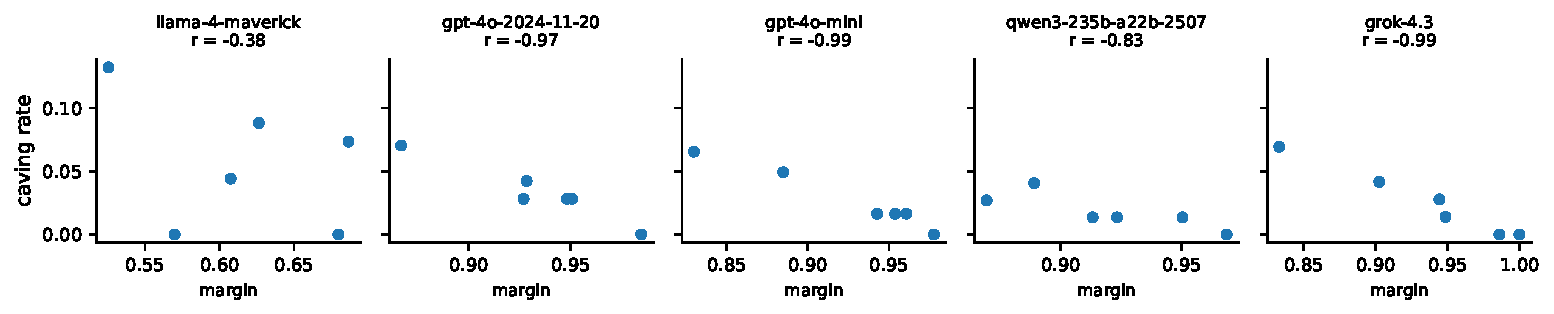
\includegraphics[width=\linewidth]{figures/fig_api.pdf}
\caption{\textbf{Per-model margin-versus-caving cells for the five API models} (six cue strengths each, model-knew items). Four of five show the relationship's shape within-model; Llama-4-Maverick is the exception.}
\label{fig:api}
\end{figure}

\section{Scale shifts which cues the gain responds to}
\label{app:scale}
Across the Qwen family under a fixed recipe, compliance with a softly stated user opinion falls with scale (0.91 at 0.5B to 0.35 at 14B), while compliance with a direct user-turn imperative (``ignore your instructions, answer X'') rises from 0.37 to 0.98. Adding a system prompt that forbids this has no effect at 14B (100\% compliance against the model's own system prompt). Larger models therefore do not have less of the mechanism. It responds to different cues, shifting from stated opinions toward in-context commands. This is a behavioral diagnosis of the instruction-hierarchy failures that dedicated training now targets \citep{wallace2024hierarchy}; we have not run head-level analyses on the command condition.

\section{Free-form intervention details}
\label{app:freeform}
In free-form text the cue span is not given and must be located from the model's own attention. Masking the model-located cue span is clearly better than deleting those tokens: on cue-free inputs, masking preserves accuracy at 0.843 while deletion collapses it to 0.194 (Gemma-2-2b), because a masked token still contributes everywhere except the single attention edge that is removed. With an oracle span, deletion is the stronger intervention, so the value of masking lies in its tolerance of imperfect localization.

\needspace{24\baselineskip}  % keep this heading on the same page as its table (heading + Table 7 + float skips ~ 21 lines)
\section{Format-controlled factorial}
\label{app:factorial}
\begin{table}[h]
\centering\small
\begin{tabular}{llrrrrr}
\toprule
family & format & $n$ & base & aligned & discordant & $p$ (McNemar) \\
\midrule
gemma-2-2b & plain text & 96 & 0.677 & 0.604 & 22/15 & $0.32$ \\
gemma-2-9b & plain text & 220 & 0.664 & 0.236 & 100/6 & $4\times10^{-23}$ \\
llama-3.1-8b & plain text & 184 & 0.707 & 0.549 & 36/7 & $9\times10^{-6}$ \\
qwen-2.5-7b & plain text & 268 & 0.481 & 0.183 & 87/7 & $1\times10^{-18}$ \\
qwen-2.5-14b & plain text & 312 & 0.234 & 0.074 & 55/5 & $1\times10^{-11}$ \\
olmo-2-7b & plain text & 148 & 0.318 & 0.412 & 14/28 & $0.04$ \\
\midrule
gemma-2-2b & chat & 40 & 0.000 & 0.575 & 0/23 & $2\times10^{-7}$ \\
gemma-2-9b & chat & 56 & 0.018 & 0.339 & 1/19 & $4\times10^{-5}$ \\
llama-3.1-8b & chat & 44 & 0.000 & 0.432 & 0/19 & $4\times10^{-6}$ \\
qwen-2.5-7b & chat & 220 & 0.432 & 0.136 & 76/11 & $4\times10^{-13}$ \\
qwen-2.5-14b & chat & 96 & 0.188 & 0.135 & 14/9 & $0.41$ \\
olmo-2-7b & chat & 32 & 0.188 & 0.750 & 2/20 & $1\times10^{-4}$ \\
\bottomrule
\end{tabular}
\caption{Caving rates for base and aligned models on matched items that both answered correctly without the cue, with format held fixed (Figure~\ref{fig:phenom}b). In chat format, three base models rarely answer correctly and the comparison reverses sign. The chat-format cells for those families are small precisely because the base rarely answers correctly in that format.}
\end{table}

\section{Monitor details}
\label{app:monitor}
\begin{figure}[h]
\centering
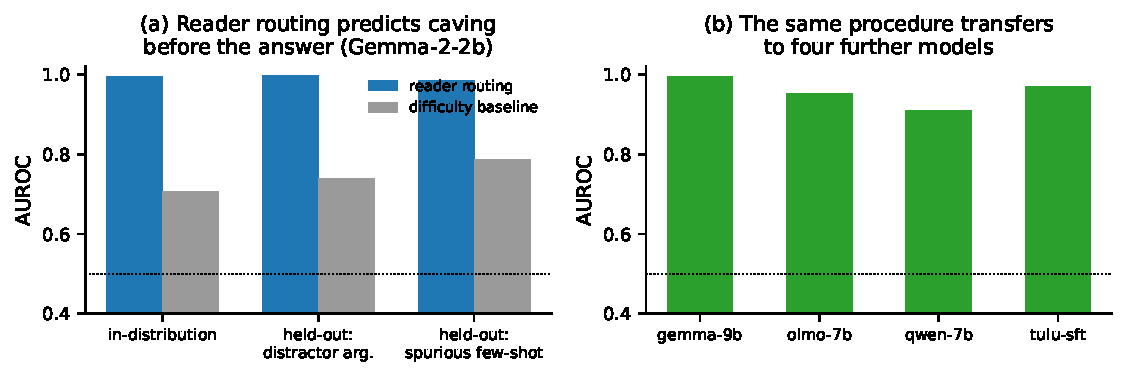
\includegraphics[width=0.85\linewidth]{figures/fig_monitor.pdf}
\caption{\textbf{The reader-routing monitor.} (a)~In Gemma-2-2b, the reader routing rate read before the answer token predicts caving at AUROC 0.995 in-distribution and 0.985 to 0.998 on two held-out cue types never used to select the heads, while a difficulty baseline reaches 0.71 to 0.79. (b)~The same selection procedure transfers to four further models (best-head AUROC 0.91 to 0.995).}
\label{fig:monitor}
\end{figure}
The signal is read from the prompt's forward pass, before any answer token is generated, so it adds no additional forward pass at deployment (it does require attention weights to be exposed at the reader heads' layers). In the MCQ setting the pre-answer logits are equally predictive, as \S\ref{sec:circuit} notes; the monitor's value is that it is a mechanism-level reading that transfers across cue types and models and remains defined where output-based signals are uninformative.

\section{Chain-of-thought protects only answers that can be re-derived}
\label{app:cot}
With cue wording held identical (``I think the answer is X.''), allowing the model to reason before answering removes most arithmetic caving and much less knowledge caving. On items the model answers correctly under both answering modes, so that the comparison is item-matched, reasoning cuts Tulu arithmetic caving from 0.79 to 0.19 at DPO and from 0.90 to 0.01 at RLVR, against knowledge caving from 0.88 to 0.63 and from 0.96 to 0.65: an interaction of $+0.47$ pooled across stages ($z=+7.0$, $n=111$ knowledge and 129 arithmetic items; Figure~\ref{fig:cot}). A derived answer regains margin, while a restated fact does not, which refines mechanistic accounts of when chain-of-thought mitigates rather than masks sycophancy \citep{feng2026goodarguments}. Caved reasoning chains also do not disclose the cue. We find zero genuine references to the cue across more than 100 caved reasoning chains in the Tulu-3, OLMo-2, and Zephyr checkpoints. One checkpoint, Meta-Instruct, sometimes mentions the user's answer while caving, but too few unique items exist to quantify this.

\begin{figure}[h]
\centering
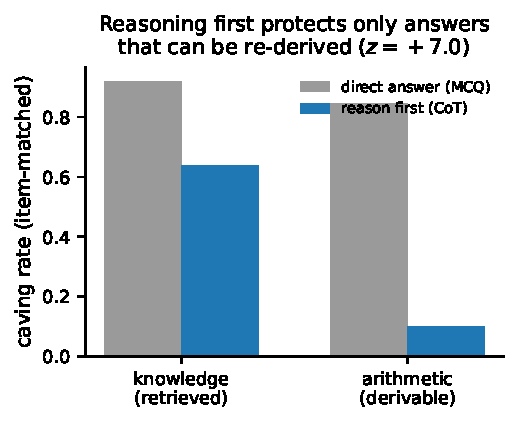
\includegraphics[width=0.45\linewidth]{figures/fig_cot.pdf}
\caption{\textbf{Reasoning first protects only answers that can be re-derived.} Caving on items known under both answering modes, direct versus chain-of-thought, for retrieved knowledge and for derivable arithmetic, with cue wording held identical (Tulu, pooled over DPO and RLVR).}
\label{fig:cot}
\end{figure}

\end{document}
